
\documentclass{beamer}
\usetheme{ucl}

%%% Increase the height of the banner: the argument is a scale factor >=1.0
%\setbeamertemplate{banner}[ucl][0.1]

%%% Change the colour of the main banner
%%% The background should be one of the UCL colours (except pink or white):
%%%   black,darkpurple,darkred,darkblue,darkgreen,darkbrown,richred,midred,
%%%   navyblue,midgreen,darkgrey,orange,brightblue,brightgreen,lightgrey,
%%%   lightpurple,yellow,lightblue,lightgreen,stone
\setbeamercolor{banner}{bg=darkpurple}
%\setbeamercolor{banner}{bg=yellow,fg=black}

%%% Add a stripe behind the banner
%\setbeamercolor{banner stripe}{bg=darkpurple,fg=black}

%%% The main structural elements
\setbeamercolor{structure}{fg=black}

%%% Author/Title/Date and slide number in the footline
\setbeamertemplate{footline}[author title date]

%%% Puts the section/subsection in the headline
% \setbeamertemplate{headline}[section]

%%% Puts a navigation bar on top of the banner
%%% For this to work correctly, the each \section command needs to be
%%% followed by a \subsection. Requires one extra compile.
% \setbeamertemplate{headline}[miniframes]
%%% Accepts an optional argument determining the width
% \setbeamertemplate{headline}[miniframes][0.3\paperwidth]


%%% Puts the frame title in the banner
%%% Won't work correctly with the above headline templates
%\useoutertheme{ucltitlebanner}
%%% Similar to above, but smaller (and puts subtitle on same line as title)
\useoutertheme[small]{ucltitlebanner}

%%% Gives block elements (theorems, examples) a border
% \useinnertheme{blockborder}
%%% Sets the body of block elements to be clear
% \setbeamercolor{block body}{bg=white,fg=black}

%%% Include CSML logo on title slide
%\titlegraphic{\includegraphics[width=0.16\paperwidth]{csml_logo}}

%%% Include CSML logo in bottom right corner of all slides
%\logo{\includegraphics[width=0.12\paperwidth]{csml_logo}}

%%% Set a background colour
% \setbeamercolor{background canvas}{bg=lightgrey}

%%% Set a background image
%%% Some sample images are available from the UCL image store:
%%%   https://www.imagestore.ucl.ac.uk/home/start
% \setbeamertemplate{background canvas}{%
%   \includegraphics[width=\paperwidth]{imagename}}



%%%%%% Some other settings that can make things look nicer
%%% Set a smaller indent for description environment
\setbeamersize{description width=2em}
%%% Remove nav symbols (and shift any logo down to corner)
\setbeamertemplate{navigation symbols}{\vspace{-2ex}}








\DeclareMathOperator{\Cov}{Cov}
\DeclareMathOperator{\Var}{Var}
\DeclareMathOperator{\E}{\mathbb{E}}
\DeclareMathOperator{\Proba}{\mathbb{P}}

\newcommand{\Covb}[2]{\ensuremath{\Cov\!\left[#1,#2\right]}}
\newcommand{\Eb}[1]{\ensuremath{\E\!\left[#1\right]}}
\newcommand{\Pb}[1]{\ensuremath{\Proba\!\left[#1\right]}}
\newcommand{\Varb}[1]{\ensuremath{\Var\!\left[#1\right]}}

% norm
\newcommand{\norm}[1]{\| #1 \|}

\newcommand{\indep}{\rotatebox[origin=c]{90}{$\models$}}





\usepackage{mathptmx,amsmath,amssymb,graphicx,bibentry,bbm,ragged2e}
\usepackage[english]{babel}

\makeatletter

\newcommand{\noun}[1]{\textsc{#1}}
\newcommand{\jitem}[1]{\item \begin{justify} #1 \end{justify} \vfill{}}
\newcommand{\sframe}[2]{\frame{\frametitle{#1} #2}}

\newenvironment{centercolumns}{\begin{columns}[c]}{\end{columns}}
%\newenvironment{jitem}{\begin{justify}\begin{itemize}}{\end{itemize}\end{justify}}



%\usetheme{Warsaw}
%\setbeamertemplate{footline}[text line]{}
%\setbeamertemplate{headline}{}
%\setbeamercolor{structure}{fg=purple!50!blue, bg=purple!50!blue}

%\setbeamersize{text margin left=15pt,text margin right=15pt}

%\setbeamercovered{transparent}


\@ifundefined{showcaptionsetup}{}{%
 \PassOptionsToPackage{caption=false}{subfig}}
\usepackage{subfig}

\usepackage[utf8]{inputenc}
\usepackage[T1]{fontenc}

\usepackage{multirow}


\makeatother

\def \draft {1}

\usepackage{xparse}
\usepackage{ifthen}
\DeclareDocumentCommand{\comment}{m o o o o}
{\ifthenelse{\draft=1}{
    \textcolor{red}{\textbf{C : }#1}
    \IfValueT{#2}{\textcolor{blue}{\textbf{A1 : }#2}}
    \IfValueT{#3}{\textcolor{ForestGreen}{\textbf{A2 : }#3}}
    \IfValueT{#4}{\textcolor{red!50!blue}{\textbf{A3 : }#4}}
    \IfValueT{#5}{\textcolor{Aquamarine}{\textbf{A4 : }#5}}
 }{}
}
\newcommand{\todo}[1]{
\ifthenelse{\draft=1}{\textcolor{red!50!blue}{\textbf{TODO : \textit{#1}}}}{}
}




\begin{document}

\title[A model of urban evolution]{A model of urban evolution based on innovation diffusion}
\author[Raimbault]{J.~Raimbault$^{1,2,3\ast}$\\\medskip
$^{\ast}$\texttt{j.raimbault@ucl.ac.uk}
}

\institute[UCL]{$^{1}$Center for Advanced Spatial Analysis, University College London\\
$^{2}$UPS CNRS 3611 Complex Systems Institute Paris\\
$^{3}$UMR CNRS 8504 G{\'e}ographie-cit{\'e}s
}


\date[July 18th 2020]{ALife 2020\\
July 18th 2020
}

\frame{\maketitle}


% The dynamics of urban systems can be understood from an evolutionary perspective, in some sense extending biological and cultural evolution. Models for systems of cities implementing elementary evolutionary processes remain however to be investigated. We propose here such a model for urban dynamics at the macroscopic scale, in which the diffusion of innovations between cities captures transformation processes (mutations) and transmission processes (diffusion), using two coupled spatial interaction models. Explorations of the model on synthetic systems of cities show the role of spatial interaction and innovation diffusion ranges on measures of diversity and utility, and the existence of intermediate ranges yielding an optimal utility. Multi-objective optimization shows how the model produces a compromize between utility and diversity. This model paves the way towards more elaborated formalizations of urban evolution.

% keywords Urban Systems; Urban Evolution; Innovation Diffusion




\section{Introduction}


%\sframe{}{
% striking intro?
%}


\sframe{Urban systems and Artificial Life}{

% Urban systems are complex as they combine technical artefacts with socio-economic dynamics at multiple temporal and spatial scales. An understanding of processes driving their dynamics is an important aspect for shaping sustainable policies, and a sustainable design and management of cities \citep{lobo2020urban}. Multiple disciplines and viewpoints have proposed such insights from a complexity perspective \citep{pumain2020conclusion}, and Artificial Life approaches have shown promising results to study urban systems, both through conceptual contributions such as interpreting cities through biological metaphors \citep{batty2009centenary}, but also through modeling and simulation for urban growth including cellular automata and evolutionary computation \citep{raimbault2020cities}.

\begin{center}
	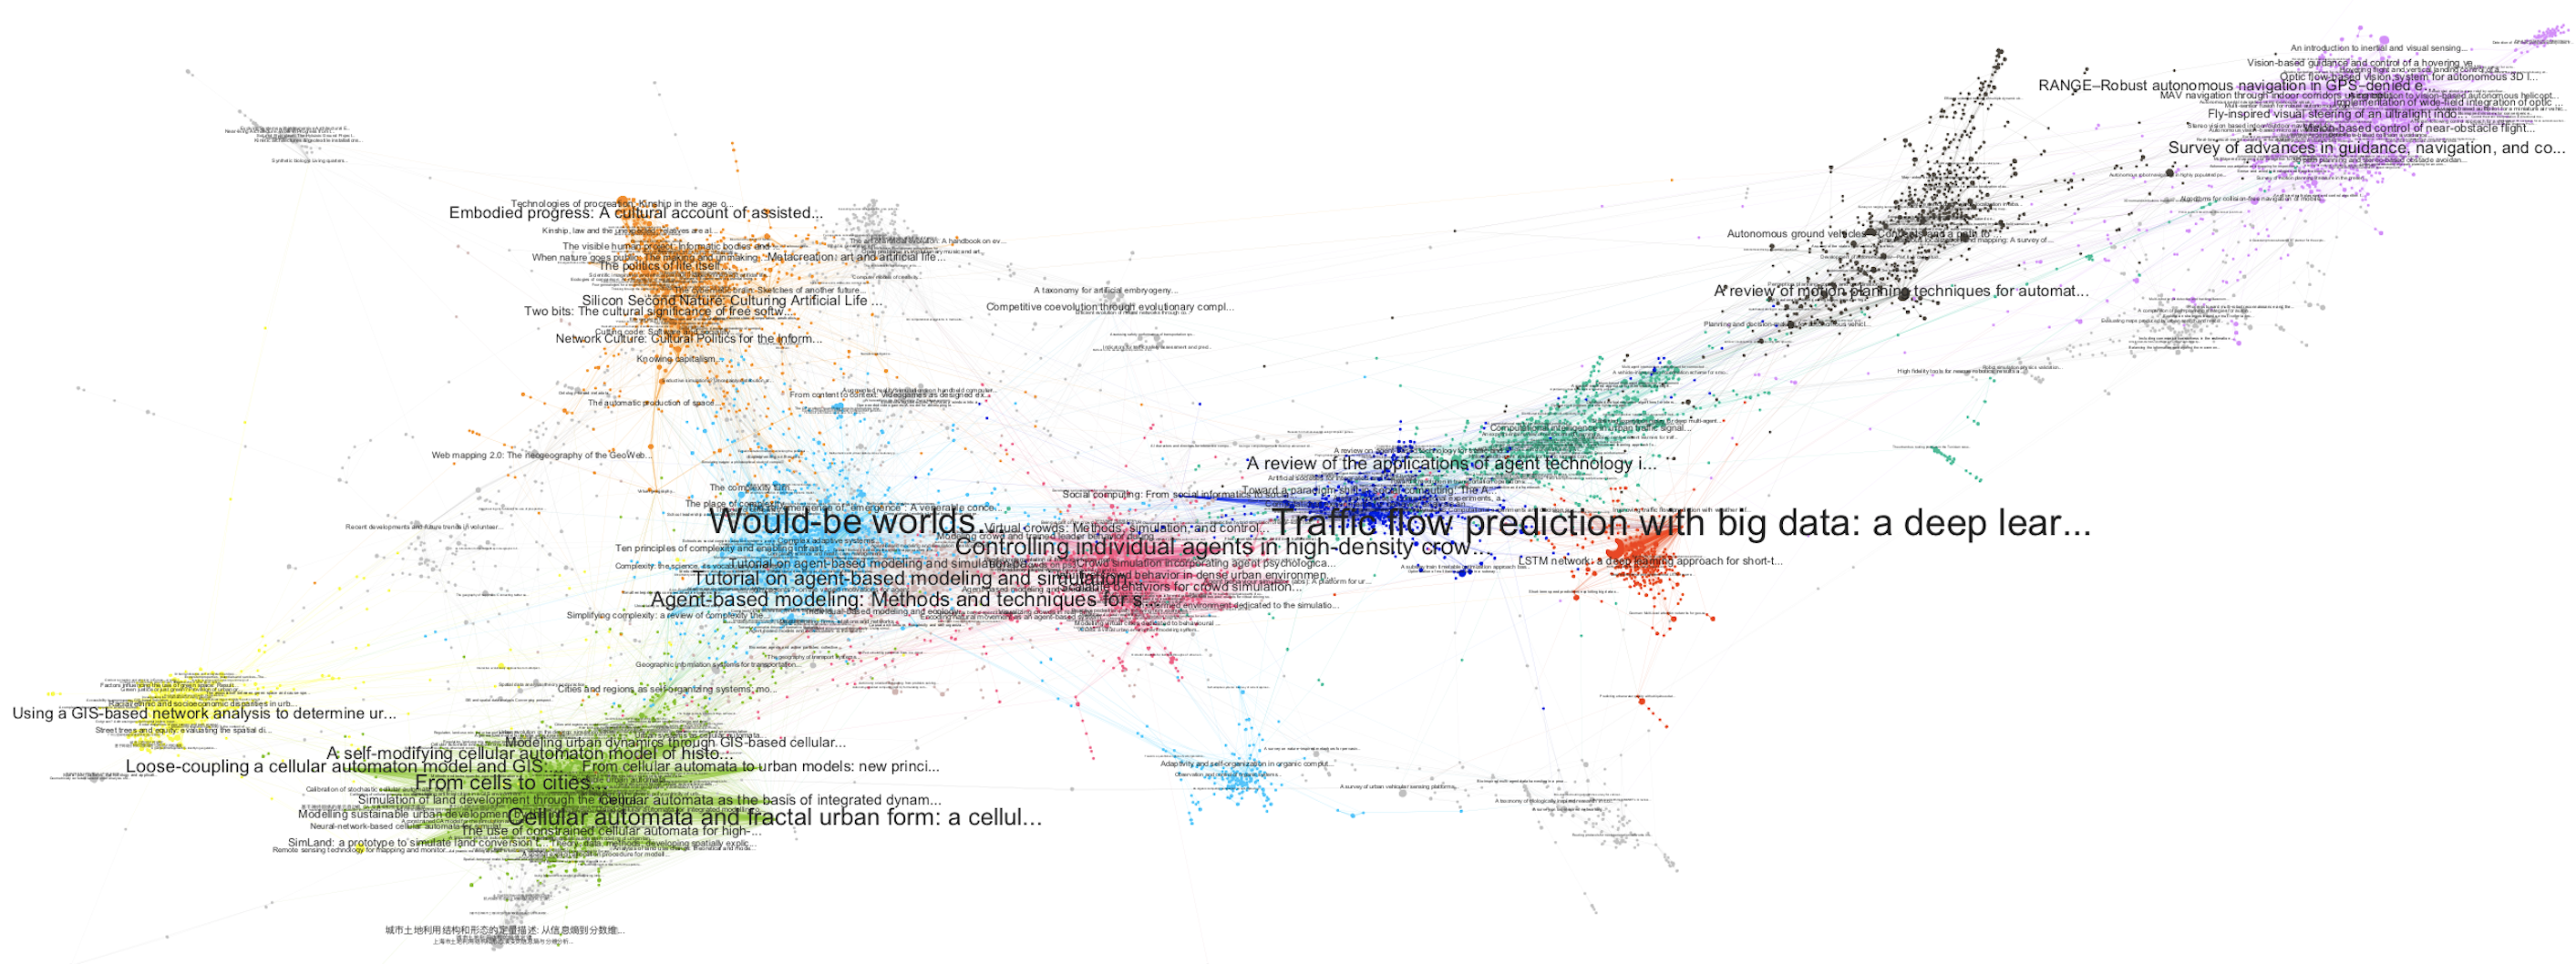
\includegraphics[width=\linewidth]{figures/corealife_zoom.png}
\end{center}

{\footnotesize \textit{Citation network of ALife studies of urban systems} \cite{raimbault2020cities} arXiv:2002.12926}

\medskip

\textbf{Transfer of concepts: } Urban morphogenesis, bio-inspired design, urban ecology, autopoiesis \cite{batty2009centenary}

}


\sframe{Urban Evolution}{

% A stream of research tightly linked to ALife relates to concepts of \emph{Urban Evolution}. These build in a sense on Cultural Evolution \citep{mesoudi2001cultural}, which aims at understanding changes in social knowledge as evolutionary processes involving replication, mutation, selection. It bears similarities with biological evolution but is not reducible to it, and for example uses the concept of \emph{meme} as transmission units comparable to genes. Both biological and cultural evolution can be linked into common frameworks and models, implying the coupling of different timescales \citep{bull2000meme}. In terms of urban studies, the concept of urban evolution is less formalized than cultural evolution and can be understood in multiple ways. \cite{votsis2019urban} use the concept of Urban DNA to characterize morphological properties of cities such as population density or the role of the road network. Similarly, \cite{kaya2017urban} describe cities based on their morphological properties as a product of their dynamics. \cite{wu2011urban} link the parameters of a cellular automaton model of urban growth to intrinsic properties of urban regions, which should play a role in their overall evolution. \cite{d2014urban} propose an urban genetic code as the way agents cooperate and compete, cities emerging as dynamical equilibria from these interactions. In Economic Geography, the concept of co-evolution is used mostly for urban agents such as firms and stakeholders \citep{gong2019co}. At the macroscopic scale of urban systems, \cite{pumain2018evolutionary} proposes an evolutionary theory to study systems of cities as complex adaptive systems, in which interactions between cities play a crucial role. Corresponding simulation models were proposed with different thematic focus, for example by \cite{cottineau2015modular} with economic exchanges and by \cite{raimbault2020indirect} with infrastructure networks. In Urban Design, \cite{batty2009digital} introduce evolutionary computation to explore possible urban forms. There still however remains a lack of models which would operationalize the concept of urban evolution in a way close to its biological and cultural counterparts, i.e. capturing explicitly the fundamental processes of transmission and transformation within differentiating subsystems \citep{durham1991coevolution}.

\textbf{Urban evolution} extending cultural evolution, cities as agents with their proper genome and evolutionary dynamics?

\medskip

\begin{center}
	\begin{columns}
	\begin{column}{0.45\linewidth}
	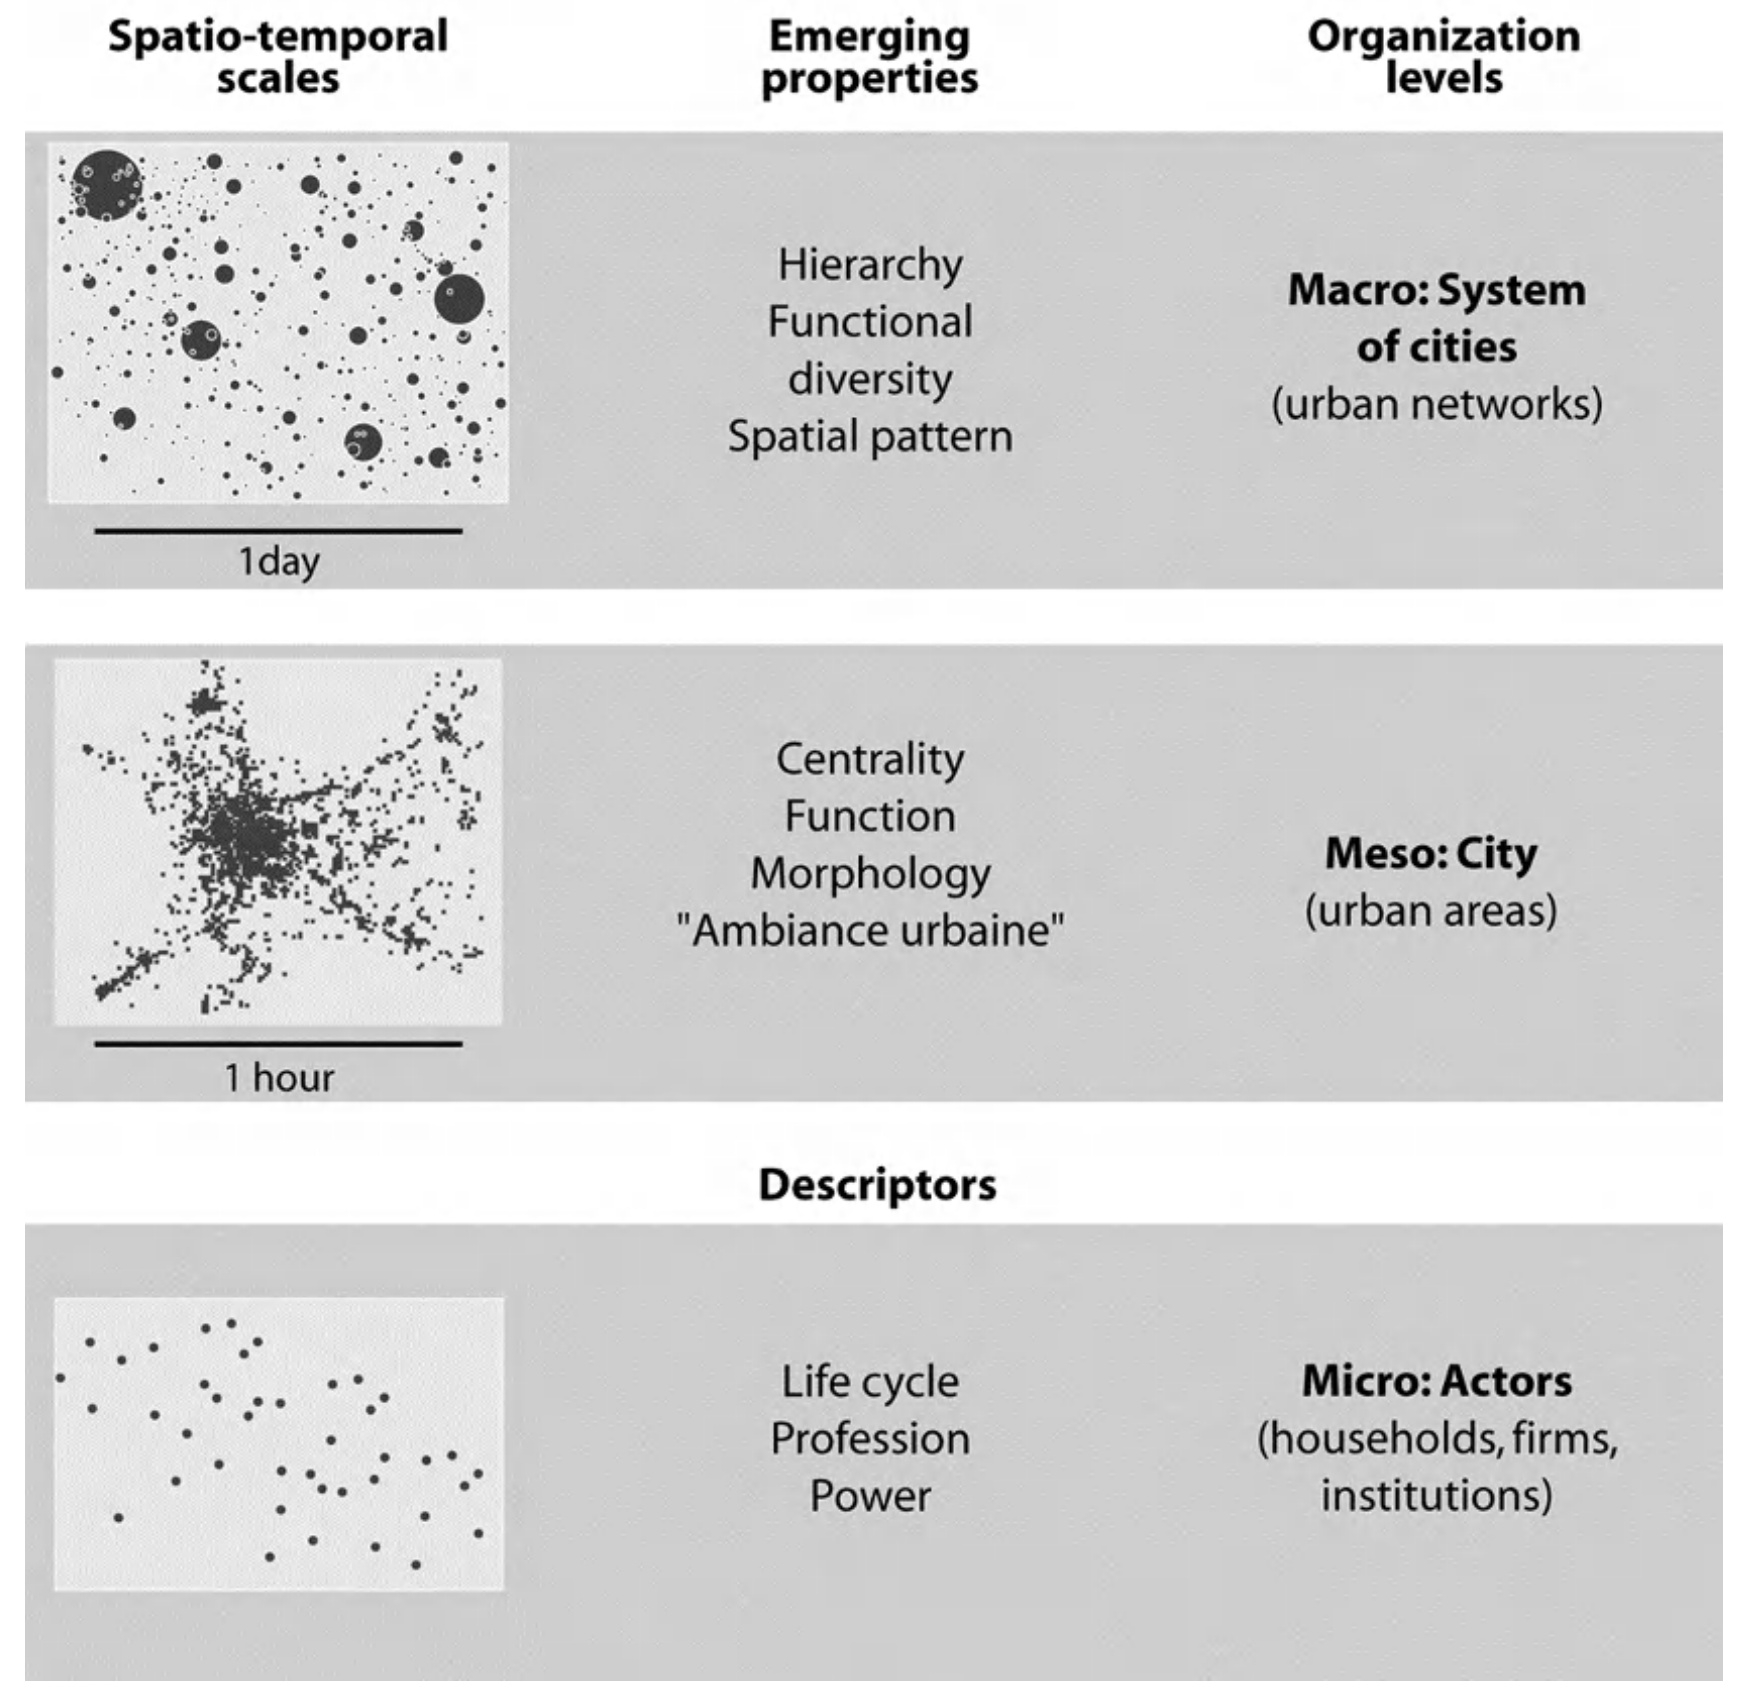
\includegraphics[width=\textwidth]{figures/evoltheory_scales.png}
	\end{column}
	\begin{column}{0.22\linewidth}
	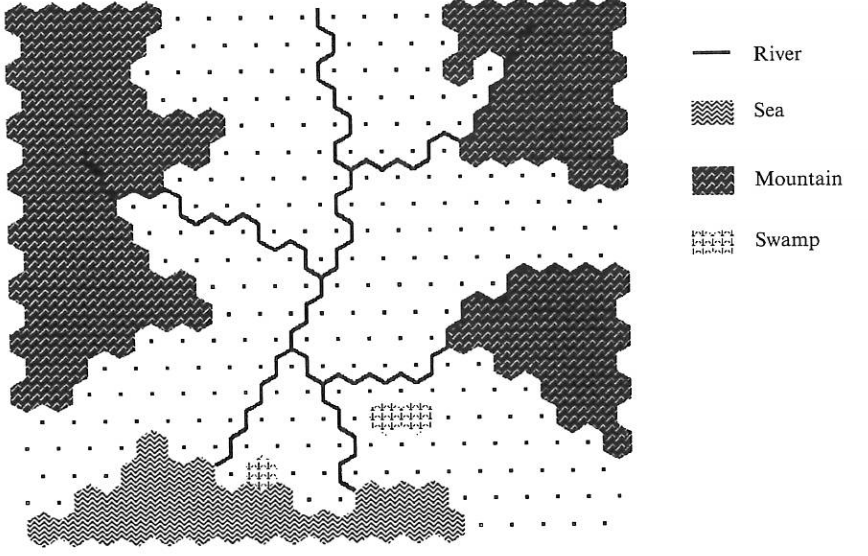
\includegraphics[width=\textwidth]{figures/simpop1.png}\\\medskip
	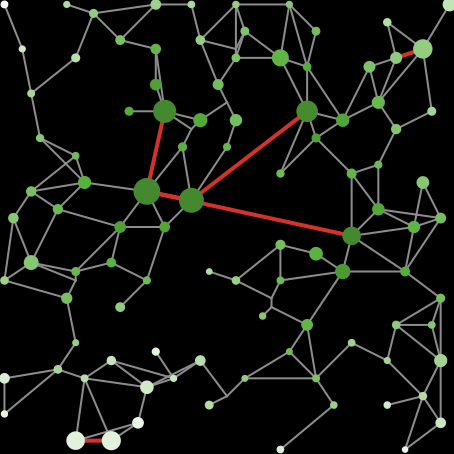
\includegraphics[width=\textwidth]{figures/setup_synth_1_tick100.png}
	\end{column}
	\end{columns}
\end{center}

\footnotesize
\textit{An evolutionary urban theory considering cities as systems within systems of cities \cite{pumain2018evolutionary}; Simpop 1 model \cite{sanders1997simpop}; SimpopNet model \cite{schmitt2014modelisation}}


}


\sframe{Innovation diffusion}{

% Besides, a central concept bridging ALife and evolution with the study of urban systems is the concept of innovation diffusion. Within artificially evolved systems, understanding how innovation emerges and how it diffuses in the population is essential \citep{bedau2000open}. One aspect of open-ended evolution are mechanisms endogeneously producing novelty. The other way around, artificial societies approaches have also been pinned as a privileged entry for understanding the dynamics of innovation \citep{zenobia2009artificial}. In the case of urban systems, \cite{hagerstrand1968innovation} had already highlighted the role of a hierarchical diffusion of innovation between cities in their trajectories. The aforementioned evolutionary urban theory suggests that innovation cycles and their hierarchical diffusion is a possible explanation for the properties of urban scaling laws \citep{pumain2006evolutionary}. \cite{paulus2004co} provides empirical support for this approach by unveiling the co-evolution between economic functions of urban areas for the French systems of cities, which are closely related to the dynamics of innovation. Evolutionary economics also study regional systems of innovation, how it diffuses and the potential existence of spatial spillovers \citep{uyarra2010evolutionary}. At the microscopic scale, several agent-based models of innovation diffusion highlight the role of social and geographical networks, both of which are embedded into urban systems \citep{zhang2019empirically}. \cite{daude2004apports} proposes for example to understand the diffusion of an agricultural innovation within a geographical system using an agent-based model. Thus, the diffusion of innovation is a privileged entry into urban evolutionary processes, as it is furthermore tightly linked with other dimensions of urban systems such as the social and economic dimensions \citep{sonis1995territorial}.

%\justify

$\rightarrow$ \textbf{Innovation diffusion} is a crucial process in artificial life evolutionary systems and open-ended evolution \cite{bedau2000open}

\medskip

$\rightarrow$ Artificial societies used to study the dynamics of innovation \cite{zenobia2009artificial}

\medskip

$\rightarrow$ Innovations diffuse hierarchically in systems of cities \cite{hagerstrand1968innovation}, potential explanation of urban scaling laws \cite{pumain2006evolutionary}

\bigskip

\textit{Innovation diffusion as a privileged entry to understand urban evolution}


}











\sframe{Research objective}{


% This paper proposes to tackle the issue of modeling urban evolution by using innovation diffusion processes to capture elementary evolutionary processes. We investigate thus the question to what extent simple models of urban evolution integrating an urban genome can be used to simulate urban dynamics. Our contribution relies on the following points: (i) we describe a relatively simple model for systems of cities at the macroscopic scales, based on population growth and the diffusion of innovation between cities; (ii) we systematically explore this model on synthetic systems of cities to extract stylized facts on different indicators including global diversity and utility.

% The rest of this paper is organized as follows: in the next section we give the model context and describe it formally. We then present numerical experiments, including internal statistical validation, exploration of the parameter space, and optimization using a multi-objective genetic algorithm. We finally discuss implications of our results and possible future extensions.


$\rightarrow$ Concepts of urban evolution do not necessarily capture essential processes (transmission and transformation) in the literature

\medskip

$\rightarrow$ Need for simple models with explicit urban genome at the system of cities scale


\bigskip
\bigskip

\textbf{Research objective: }

\medskip

\textit{Describe and systematically explore an urban evolution model based on innovation diffusion, for urban dynamics at the macroscopic scale}


}



\section{Model description}


\sframe{Model rationale}{

% The core idea of the model is to build on a concept of ``Urban DNA'' which would capture evolution processes as in biological evolution and cultural evolution, i.e. a kind of genome that cities would be exchanging and which would undergo mutation processes. A suitable candidate is to build on the concept of \emph{meme} introduced in the field of cultural evolution. However, several particularities must be stressed out when working with urban systems. First, they are multi-dimensional implying very different types of agents, including physical and technical artefacts (e.g. infrastructures) but also social and economical structures. A comprehensive urban genome would include these very different dimensions. Then, they are multi-scalar in time and space, meaning that evolution processes, if they exist, may occur at different paces and through different elementary carriers. Finally, they are embedded in the geographical space, what structures the way transmission and mutation can occur, but also can strongly change properties of underlying processes \citep{raimbault2019space}. We choose to focus on the last point, considering a model at the macroscopic scale where cities are agents and with a one-dimensional genome, but in which spatial interactions are crucial for the dynamics. More particularly, this model combines two spatial interaction models \citep{fotheringham1989spatial}.


%Several models have been proposed to simulate the diffusion of innovation at microscopic and mesoscopic scales \citep{kiesling2012agent}. \cite{blommestein1987adoption} describe a model of innovation diffusion and urban dynamics with endogenous demand for innovations, but in which the spatial component only influences prices of innovations. \cite{deffuant2005individual} give an example of an elaborated model for adoption dynamics at the microscopic level. Effective channels for the diffusion of innovations are multiple, and can for example be urban firm linkages \citep{rozenblat2007firm}. \cite{pumain2017simpoplocal} describe a model based on innovation diffusion to explain the emergence of the first cities. \cite{favaro2011gibrat} study an urban growth model including innovation diffusion at the scale of the urban system. Our model builds on this last framework, extending and adapting it to an urban evolution context. We keep the innovation diffusion and spatial interaction processes unchanged, but take a deterministic update of populations. The introduction of new innovations is modified to better fit the urban evolution context. Finally, the introduction of indicators to quantify model behavior regarding different dimensions is a significant extension to the initial model.

%In our model, cities are characterized by their size in terms of population. City sizes evolve following a spatial interaction model taking into account the attractivity of cities. This attractivity is determined by how innovative cities are. Transformation processes are included as mutations, when random innovations appear in cities. Transmission processes (spatial crossover) are included by diffusing innovations between cities. Finally, the existence of subsystems in which evolution can occur comes naturally with the spatial aspect of the model: different regions in space may behave and evolve differently, possibly resulting in the emergence of co-evolution niches \citep{holland2012signals,raimbault2018co}.

\begin{itemize}
	\item Agents are cities, macroscopic scale (regional, country, continental) and long time scales (century)
	\item Cities characterized by their size in terms of population; genome as adoption proportions of innovations (social or technological) for each city (one single dimension to simplify)
	\item Following \cite{favaro2011gibrat}, attractivity of cities due to level of innovation drive their population growth through spatial interactions; innovation diffuse through an other spatial interaction model \cite{fotheringham1989spatial}
	\item Mutations occur in cities as new innovations appear
\end{itemize}


}



\sframe{Model description}{

% step by step scheme ?


\begin{pspicture}(0,-2.94)(11.17,2.94)
\definecolor{colour0}{rgb}{1.0,0.2,0.0}
\definecolor{colour1}{rgb}{0.2,0.8,0.0}
\definecolor{colour2}{rgb}{0.0,0.8,1.0}
\pscircle[linecolor=black, linewidth=0.04, dimen=outer](0.8,0.26){0.8}
\pscircle[linecolor=black, linewidth=0.04, dimen=outer](3.44,-1.9){0.38}
\pscircle[linecolor=black, linewidth=0.04, dimen=outer](4.64,2.08){0.5}
\pscircle[linecolor=black, linewidth=0.04, dimen=outer](6.72,-2.12){0.48}
\rput[bl](0.12,1.1){\textit{City 1}}
\rput[bl](4.16,2.64){\textit{City 2}}
\rput[bl](2.88,-2.66){\textit{City 3}}
\rput[bl](6.16,-2.94){\textit{City 4}}
\pscircle[linecolor=black, linewidth=0.04, dimen=outer](7.56,2.48){0.44}
\pscircle[linecolor=black, linewidth=0.04, dimen=outer](7.56,2.38){0.34}
\pscircle[linecolor=black, linewidth=0.04, dimen=outer](7.56,2.28){0.22}
\rput[bl](8.18,2.18){Population}
\psframe[linecolor=black, linewidth=0.04, fillstyle=solid,fillcolor=colour0, dimen=outer](7.66,1.56)(7.4,1.22)
\psframe[linecolor=black, linewidth=0.04, fillstyle=solid,fillcolor=colour1, dimen=outer](7.66,1.74)(7.4,1.54)
\psframe[linecolor=black, linewidth=0.04, fillstyle=solid,fillcolor=colour2, dimen=outer](7.66,1.94)(7.4,1.72)
\rput[bl](8.14,1.46){Innovation genome}
\psframe[linecolor=black, linewidth=0.04, fillstyle=solid,fillcolor=colour0, dimen=outer](0.82,0.2)(0.56,-0.38)
\psframe[linecolor=black, linewidth=0.04, fillstyle=solid,fillcolor=colour0, dimen=outer](4.72,2.2)(4.52,1.72)
\psframe[linecolor=black, linewidth=0.04, fillstyle=solid,fillcolor=colour0, dimen=outer](6.74,-1.94)(6.54,-2.44)
\psframe[linecolor=black, linewidth=0.04, fillstyle=solid,fillcolor=colour0, dimen=outer](3.48,-1.8)(3.3,-2.16)
\psframe[linecolor=black, linewidth=0.04, fillstyle=solid,fillcolor=colour1, dimen=outer](0.82,0.58)(0.56,0.18)
\only<2->{
\psframe[linecolor=black, linewidth=0.04, fillstyle=solid,fillcolor=colour1, dimen=outer](4.72,2.4)(4.52,2.18)
\psframe[linecolor=black, linewidth=0.04, fillstyle=solid,fillcolor=colour1, dimen=outer](3.48,-1.6)(3.3,-1.82)
\psframe[linecolor=black, linewidth=0.04, fillstyle=solid,fillcolor=colour1, dimen=outer](6.74,-1.76)(6.54,-1.98)
\psline[linecolor=colour1, linewidth=0.04, linestyle=dashed, dash=0.17638889cm 0.10583334cm, arrowsize=0.05291667cm 2.0,arrowlength=1.4,arrowinset=0.0]{<-}(4.08,2.08)(1.4,0.84)
\psline[linecolor=colour1, linewidth=0.04, linestyle=dashed, dash=0.17638889cm 0.10583334cm, arrowsize=0.05291667cm 2.0,arrowlength=1.4,arrowinset=0.0]{<-}(6.16,-2.1)(1.48,-0.14)
\psline[linecolor=colour1, linewidth=0.04, linestyle=dashed, dash=0.17638889cm 0.10583334cm, arrowsize=0.05291667cm 2.0,arrowlength=1.4,arrowinset=0.0]{<-}(3.06,-1.74)(1.2,-0.44)
\psline[linecolor=colour1, linewidth=0.04, linestyle=dashed, dash=0.17638889cm 0.10583334cm, arrowsize=0.05291667cm 2.0,arrowlength=1.4,arrowinset=0.0]{<-}(7.98,0.5)(7.1,0.5)
\rput[bl](8.14,0.4){Innovation diffusion}
}
\only<3->{
\psline[linecolor=black, linewidth=0.08, arrowsize=0.05291667cm 2.0,arrowlength=1.4,arrowinset=0.0]{<->}(1.56,0.5)(4.18,1.74)
\psline[linecolor=black, linewidth=0.16, arrowsize=0.05291667cm 2.0,arrowlength=1.4,arrowinset=0.0]{<->}(1.6,0.04)(6.2,-1.88)
\psline[linecolor=black, linewidth=0.08, arrowsize=0.05291667cm 2.0,arrowlength=1.4,arrowinset=0.0]{<->}(4.88,1.62)(6.46,-1.6)
\psline[linecolor=black, linewidth=0.04, arrowsize=0.05291667cm 2.0,arrowlength=1.4,arrowinset=0.0]{<->}(1.44,-0.32)(3.16,-1.54)
\psline[linecolor=black, linewidth=0.04, arrowsize=0.05291667cm 2.0,arrowlength=1.4,arrowinset=0.0]{<->}(3.86,-1.94)(6.2,-2.22)
\psline[linecolor=black, linewidth=0.04, arrowsize=0.05291667cm 2.0,arrowlength=1.4,arrowinset=0.0]{<->}(7.06,0.96)(7.96,0.96)
\psline[linecolor=black, linewidth=0.08, arrowsize=0.05291667cm 2.0,arrowlength=1.4,arrowinset=0.0]{<->}(3.7,-1.5)(4.62,1.5)
\rput[bl](8.12,0.84){Population growth}
}
\only<4->{
\psframe[linecolor=black, linewidth=0.04, fillstyle=solid,fillcolor=colour2, dimen=outer](0.82,0.94)(0.56,0.56)
\pscircle[linecolor=colour2, linewidth=0.04, linestyle=dashed, dash=0.17638889cm 0.10583334cm, dimen=outer](0.81,0.27){0.72}
\pscircle[linecolor=colour2, linewidth=0.04, linestyle=dashed, dash=0.17638889cm 0.10583334cm, dimen=outer](7.6,-0.08){0.26}
\rput[bl](8.14,-0.18){Mutation}
}
\end{pspicture}



}


\sframe{Model formalization}{

% We now formally describe the urban evolution model. A number $N$ of cities are located in the geographical space, and described in time by their size $P_i (t)$ (which generally corresponds to population). The geography is captured with a distance matrix $d_{ij}$ between cities. We consider a one-dimensional technological space in which innovations can be introduced, indexed by their order of apparition $c$. Cities are then also characterized by their innovation profile $\delta_{c,i} (t) \in \left[0;1\right]$ which represents the proportion of population having adopted innovation $c$ in the city $i$ at time $t$. We assume exclusivity in the adoption of innovation, i.e. that we always have $\sum_c \delta_{c,i} (t) = 1$. This innovation profile corresponds to the urban genome. Each innovation has furthermore a utility $u_c >0$ which will influence its diffusion dynamics.


%Starting from an initial configuration, the simulation model is iterated in time with the following steps at each time tick:

%	\item The crossover between urban genomes relies on spatial processes of innovation diffusion. This means that existing innovations are propagated between cities following a spatial interaction model given by

%\begin{equation}
%\delta_{c,i,t} = \frac{\sum_j p_{c,j,t-1}^{\frac{1}{u_c}} \cdot \exp{(-\frac{d_{ij}}{d_I})}}{\sum_c \sum_j p_{c,j,t-1}^{\frac{1}{u_c}} \cdot \exp{(-\frac{d_{ij}}{d_I})}}
%\end{equation}

%where $p_{c,i,t} = \delta_{c,i,t} \cdot \frac{P_{i}(t)}{\sum_k P_k (t)}$ is the share of total population adopting $c$ in the city $i$ at time $t$; $d_I$ is the characteristic distance in the spatial innovation model, for which an increase will correspond to a broader spatial diffusion. As the population share is between 0 and 1, higher utilities will effectively diffuse faster as the exponent $1/u_c$ is used. In other terms, the inverse of the utility is the coefficient of population in the underlying spatial interaction model, and using an exponent is more relevant in that sense.

%	\item The sizes of cities evolve according to their performance in terms of innovation, i.e. more innovative cities are more attractive. This stage is also deterministic, following  with $P_i(t) - P_i(t-1) = w_I\cdot \sum_j \frac{V_{ij}}{<V_{ij}>}$ where $w_I$ is a fixed growth rate, and where the interaction potential is defined by
%\begin{equation}
%V_{ij}= \frac{P_{i}(t-1) \cdot P_{j}(t-1)}{(\sum_k P_k(t-1))^2} \cdot \exp{\left(-\frac{d_{ij}}{d_G} \cdot \prod_c \delta_{c,i,t}^{\phi_{c,t}}\right)}
%\end{equation}
%where $\phi_{c,t} = \sum_i \delta_{i,c,t}\cdot P_i(t-1) /\sum_{i,c} \delta_{i,c,t}\cdot P_{i}(t-1)$ is the macroscopic adoption level (globally more adopted innovations will have a higher attractivity); $d_G$ is the characteristic distance for this second spatial interaction model. This model for population dynamics was proposed in such a setting by \citep{raimbault2020indirect} without the additional innovation attractivity term.

% \item Finally, mutations in the urban genome (transformation process) corresponds to the introduction of new innovations. Each city has an innovation activity $\beta$ independent of its size, which corresponds to an intrinsic mutation rate; and will have a probability to innovate function of its size, similar to a Gibrat model \citep{pumain2012theorie}, as $\beta \cdot \left(P_i (t) / \max_k P_k (t)\right)^{\alpha_I}$ where $\alpha_I$ is a hierarchy exponent biasing the innovation towards larger cities. The utility for a new innovation is drawn stochastically, following either a normal or log-normal distribution, such that (i) its average corresponds to the current mean of utilities for existing innovations, and (ii) its standard deviation is a fixed parameter $\sigma_U$, which allows controlling the ``disruptivity'' of innovations. Urban genomes are modified such that the new innovation has an initial penetration rate $r_0$ in the innovative city (previous innovation shares are rescaled for this city).

%The urban evolution is stopped after a fixed number of steps $t_f$. Note that other stopping criteria such as reaching a total population, a maximal population for the largest city, or a maximal number of innovations introduced, could be included for other applications of the model.

\footnotesize

At each time step, with $P_i \left(t\right)$ population, $\delta_{c,i}\left(t\right)$ genome, $u_c$ utility of innovation, $p_{c,i,t}$ share of total population adopting innovation $c$ in city $i$
\begin{enumerate}
	\item Crossover through the diffusion of innovations
	\[
	\delta_{c,i,t} \textrm{ = } \frac{\sum_j p_{c,j,t-1}^{\frac{1}{u_c}} \cdot \exp{\left(-\frac{d_{ij}}{d_I}\right)}}{\sum_c \sum_j p_{c,j,t-1}^{\frac{1}{u_c}} \cdot \exp{\left(-\frac{d_{ij}}{d_I}\right)}}	
	\]
	\item Population growth through spatial interactions $P_i\left(t\right) - P_i\left(t-1\right) \textrm{ = } w_I\cdot \sum_j \frac{V_{ij}}{<V_{ij}>}$ with
	\[ 
	V_{ij} \textrm{ = } \frac{P_{i}\left(t-1\right) \cdot P_{j}\left(t-1\right)}{\left(\sum_k P_k\left(t-1\right)\right)^2} \cdot \exp{\left(-\frac{d_{ij}}{d_G} \cdot \prod_c \delta_{c,i,t}^{\phi_{c,t}}\right)}
	\]
	and $\phi_{c,t} \textrm{ = } \sum_i \delta_{i,c,t}\cdot P_i\left(t-1\right) /\sum_{i,c} \delta_{i,c,t}\cdot P_{i}\left(t-1\right)$
	\item Mutations with innovations introduced with probability $\beta \cdot \left(P_i \left(t\right) / \max_k P_k \left(t\right)\right)^{\alpha_I}$ and an initial penetration rate $r_0$; new utility $u_c$ randomly distributed (normal or log-normal) with average current average utility and standard deviation a given parameter $\sigma_U$
\end{enumerate}



}


\sframe{Model indicators}{

% The behavior of the model is quantified through indicators at the macroscopic scale. These should allow extracting stylized facts from the model exploration. We consider the following indicators:
%	\item Average diversity, defined as an Herfindhal diversity index over innovation shares across cities, averaged in time as
%	\begin{equation}
%		D = \frac{1}{t_f + 1} \sum_{t=0}^{t_f} \left(1 - \sum_{i,c} \left(p_{c,i,t}\right)^2 \right)	
%	\end{equation}
%	Note that other diversity indices could be applied, or a similar be computed on macroscopic adoption shares or within each city, and would yield different results. This one has the advantage to combine the diversity within and across cities.
%	\item Average utility, given by the weighted average of innovation utilities, averaged in time, as
%	\begin{equation}
%		U = \frac{1}{t_f + 1} \sum_{t=0}^{t_f} \sum_{i,c} \delta_{c,i,t} u_c 
%	\end{equation}
%	\item Innovativity, given by the average number of innovations per city and unit of time $I = \frac{\max c}{N\cdot (t_f + 1)}$.
%	\item To quantify the trajectories of city populations, many indicators can be used \citep{raimbault2020unveiling}. We choose to simply quantify the level of hierarchy of final populations. It is estimated by adjusting a rank-size law for populations, using an Ordinary Least Squares regression on logarithms of populations as a function of logarithms of ranks. This captures if the urban systems has become more unequal in terms of population balance, since the initial hierarchy is fixed.

\begin{itemize}
	\item Average diversity
	\[
	D \textrm{ = } \frac{1}{t_f \textrm{+} 1} \sum_{t\textrm{=}0}^{t_f} \left(1 - \sum_{i,c} \left(p_{c,i,t}\right)^2 \right)	
	\]
	\item Average utility
	\[
	U \textrm{ = } \frac{1}{t_f \textrm{ + } 1} \sum_{t \textrm{=}0}^{t_f} \sum_{i,c} \delta_{c,i,t} u_c 
	\]
	\item Innovatitivity 
	\[
	I \textrm{ = } \frac{\max c}{N\cdot \left(t_f \textrm{ + } 1\right)}
	\]
	\item Population trajectories, summarized by final hierarchy \cite{raimbault2020unveiling}
\end{itemize}



}



\sframe{Synthetic configurations}{

% Although \cite{raimbault:halshs-01880492} proposed to apply the model of \cite{favaro2011gibrat} on real systems of cities, we focus our model study here on synthetic systems of cities, in order to isolate intrinsic effects independently of geographical contingencies. Cities are located randomly in an uniform square space. City sizes follow a Zipf law with exponent $\alpha_0 = 1$, i.e. such that $P_i (0) = \frac{P_{max}}{i^{\alpha_0}}$ \citep{pumain2012theorie}. We do not modify this initial hierarchy in our experiments. Distances between cities $d_{ij}$ are computed as euclidian distances. We take $N=30$ cities, $P_{max} = 10^5$ and $t_f = 50$ in our experiments, corresponding to a regional or small national system of cities, on timescales of the order of a century. According to these approximates scales, we fix $w_I = 0.005$ in experiments which gives a maximal possible growth factor of $(1.005)^{50} = 1.28$ over the whole period, in consistence with mature urban systems having relatively slow population growth \citep{pumain1982dynamique}.

Model applied on synthetic systems of cities (so that conclusions are independent of geographical contingencies \cite{raimbault2019space}):

\medskip

\begin{itemize}
	\item random positions and rank-size hierarchy $P_i \left(0\right) \textrm{ = } \frac{P_{max}}{i^{\alpha_0}}$ with $\alpha_0 \textrm{ = } 1.0$ and $P_{max} \textrm{ = } 100,000$
	\item regional urban system scale: $N \textrm{ = } 30$ cities
	\item simulated for $t_f \textrm{ = } 50$ macroscopic time steps (order of magnitude of a century)
\end{itemize}



}



\sframe{Model parameters}{

\centering

% Parameter explored in experiments are the spatial interaction parameters $d_G,d_I \in \left[0;2\right]$ which correspond to the crossover mechanism; and the innovation parameters which correspond to the mutation mechanism: innovation rate $\beta \in \left[0;1\right]$, innovation hierarchy $\alpha_I \in \left[0;2\right]$, innovation utility standard deviation $\sigma_U \in \left[ 0.7;2\right]$ (the lower bound is a constraint for the existence of the log-normal with log mean 0), initial penetration rate $r_0 \in \left[0.1;0.9\right]$, and type of innovation utility as normal or log-normal. All model parameters are summarized in Table~\ref{tab:params}, with their range, default value and associated process.

%\caption{Summary of model parameters. We first describe synthetic setup parameters which are fixed during our experiments, and then parameters varied during experiments. We give associated process, indicative range and default value for each parameter.\label{tab:params}}\medskip
%	\hspace{-1cm}
%	\footnotesize

	\begin{tabular}{|l|l|l|l|l|l|}
	\hline
	Parameter & Not. & Process & Range & Def. \\ \hline
	Number of cities & $N$ & Spatial scale & $[10 ; 100]$ & $30$\\
	Initial hierarchy & $\alpha_0$ & System of cities & $[0.5 ; 2.0]$ & $1$\\
	Initial population & $P_{max}$ & System of cities & $[10^4 ; 10^7]$ & $10^5$\\
	Simulation steps & $t_f$ & Temporal scale & $[10 ; 100]$ & $50$\\
	Growth rate & $w_I$ & Pop. growth & $[0.001 ; 0.01]$ & $0.005$\\\hline
	Gravity range & $d_G$ & Crossover & $[0 ; 2]$ & $1$\\
	Innovation range & $d_I$ & Crossover & $[0 ; 2]$ & $1$\\
	Innovation rate & $\beta$ & Mutation & $[0 ; 1]$ & $0.5$\\
	Innovation hierarchy & $\alpha_I$ & Mutation & $[0 ; 2]$ & $1$\\
	Innov. utility std. & $\sigma_U$ & Mutation & $\left[ 0.7;2\right]$ & $1$\\
	Penetration rate & $r_0$ & Mutation & $\left[0.1;0.9\right]$ & $0.5$\\
	Utility type & - & Mutation & \{n;ln\}& ln \\
	\hline
	\end{tabular}



}



\section{Results}


\sframe{Implementation}{

% The model is implemented in \texttt{scala} and integrated into the OpenMOLE software \citep{reuillon2013openmole} for numerical experiments. OpenMOLE allows embedding models in any language as black boxes, provides a transparent access to high performance computing infrastructures, and model exploration and validation methods such as sensitivity analysis, design of experiments, and calibration methods. Experiments are designed through workflows using a Domain Specific Language \citep{passerat2017reproducible}.

%Source code of the model and analysis, and results are available on the open git repository of the project at \url{https://github.com/JusteRaimbault/UrbanEvolution}. Simulation data files are available on the dataverse repository at \url{https://doi.org/10.7910/DVN/Q5GKZ0}.

%\footnotesize
\justify



Model implemented in \texttt{scala}; relatively large parameter space

\medskip

$\rightarrow$ integration into the OpenMOLE model exploration open source software \cite{reuillon2013openmole}

\begin{center}

\includegraphics[height=0.13\textheight]{figures/iconOM.png}

\includegraphics[height=0.13\textheight]{figures/openmole.png}
\end{center}


\textit{Enables seamlessly (i) model embedding; (ii) access to HPC resources; (iii) exploration and optimization algorithms}

\medskip

\url{https://openmole.org/}


}




\sframe{Statistical consistency}{


%As the model is stochastic through the mutation process, first experiments are needed to assess the ``internal validity'' of the model, i.e. to what extent studied indicators are robust to noise and how much stochastic repetitions are needed to significantly distinguish between central values of distributions for different parameter points. We sample thus 100 parameter points using a Latin Hypercube Sampling, and run 1000 model repetitions for each point, in order to estimate the statistical properties across different points in the parameter space.

%The Sharpe ratios estimated on repetitions as sample standard deviation relative to absolute sample mean have high values for all indicators (min. 3.9 and median 12.1 for diversity; min. 3.0 and median 6.2 for innovation; min. 1.7 and median 3.6 for utility; min. 26 and median 257.3 for population hierarchy). This implies that stochastic noise is not an issue for interpreting indicator values.

%We also study the distance between points averages relative to their standard deviation, in order to know the significance in comparing averages. This distance is defined by $\Delta_{ij} = 2\frac{\left|\mu_i - \mu_j \right|}{\sigma_i + \sigma_j}$ if $\mu_i$ are estimated central values (mean or median) and $\sigma_i$ estimated standard deviations. These distances have an average and median larger than one for all couples, and a first quartile larger than one for innovation and population hierarchy, while the first quartile is 0.5 for utility and 0.6 for diversity. The most constraining indicators in terms of statistical precision are thus utility and diversity. As in the case of normal distributions, a 95\% confidence interval of size $\sigma_2$ is achieved for $n\simeq 64$ runs, a number of 50 runs is satisfying for further experiments.

\begin{itemize}
	\item Latin Hypercube Sampling of 100 parameter points, 1000 replications for each
	\item Sharpe ratios have high values for all indicators and all parameters (minimum 1.7 for utility)
	\item Average and median relative distances defined as $\Delta_{ij} \textrm{ = } 2\frac{\left|\mu_i - \mu_j \right|}{\sigma_i \textrm{ + } \sigma_j}$ larger than one for all indicators: 50 repetitions in further experiments
\end{itemize}




}


\sframe{Model exploration: diversity}{

% We then explore a grid of the parameter space consisting of 23,168 parameter points, with a finer step on spatial parameters $d_G$ and $d_I$, and with 50 model replications for each parameter point. We find that the type of distribution for utility has small effects for all indicators and across most parameter values, but particular cases are more interesting in the log-normal case, which we comment further. Similarly, the effect of innovation hierarchy $\alpha_I$ and of innovation utility standard deviation $\sigma_U$ do not seem to induce strong qualitative differences, so we discuss model behavior obtained at $\alpha_I = 1$ and $\sigma_U = 1$.

% The Fig.~\ref{fig:exploration} shows the behavior of indicators with remaining parameters varying, namely spatial interaction parameters $d_G$ and $d_I$, mutation rate $\beta$ and innovation adoption $r_0$. Regarding the behavior of diversity (top left panel of Fig.~\ref{fig:exploration}), we find that it always increases for larger population growth spatial interaction distances, meaning that broader population exchanges will induce a higher diversity in innovations, probably through the higher innovation dynamics induced. This increase is however slowed down around half of the width of the world ($d_G = 0.5$), which is more obvious with higher values of mutation rates for which a plateau is reached (bottom row, in particular the sub-panel for $r_0=0.1$ and $\beta = 0.5$): higher intrinsic innovation dampens the role of spatial interactions. An increase of innovation interaction distance $d_I$ on the contrary monotonously decreases diversity, consistently with the idea of local innovation niches which can be overridden by competing innovations of higher utility coming from further away. Finally, mutation rate has a strong quantitative impact on total diversity as expected, while higher early adoption rate will change diversity behavior only when mutation rates are also high.

%	\caption{Values of indicators obtained with the grid model exploration. Each plot give each indicator among diversity $D$, utility $U$, innovation $I$ and population hierarchy $\alpha_P$, at fixed parameters $\alpha_I = 1$, $\sigma_U = 1$ and for the log-normal utility law. Indicators are plotted as a function of gravity interaction range $d_G$, for varying values of innovation diffusion range $d_I$ (color). Sub-panels show varying values of mutation rate $\beta$ (rows) and of early adoption rate $r_0$ (columns).\label{fig:exploration}}

Grid sampling of the parameter space (23,168 points, 50 replications) with a finer grid on $d_G$ and $d_I$; plots shown at $\alpha_I \textrm{ = } 1$ and $\sigma_U \textrm{ = } 1$

\medskip

\begin{center}
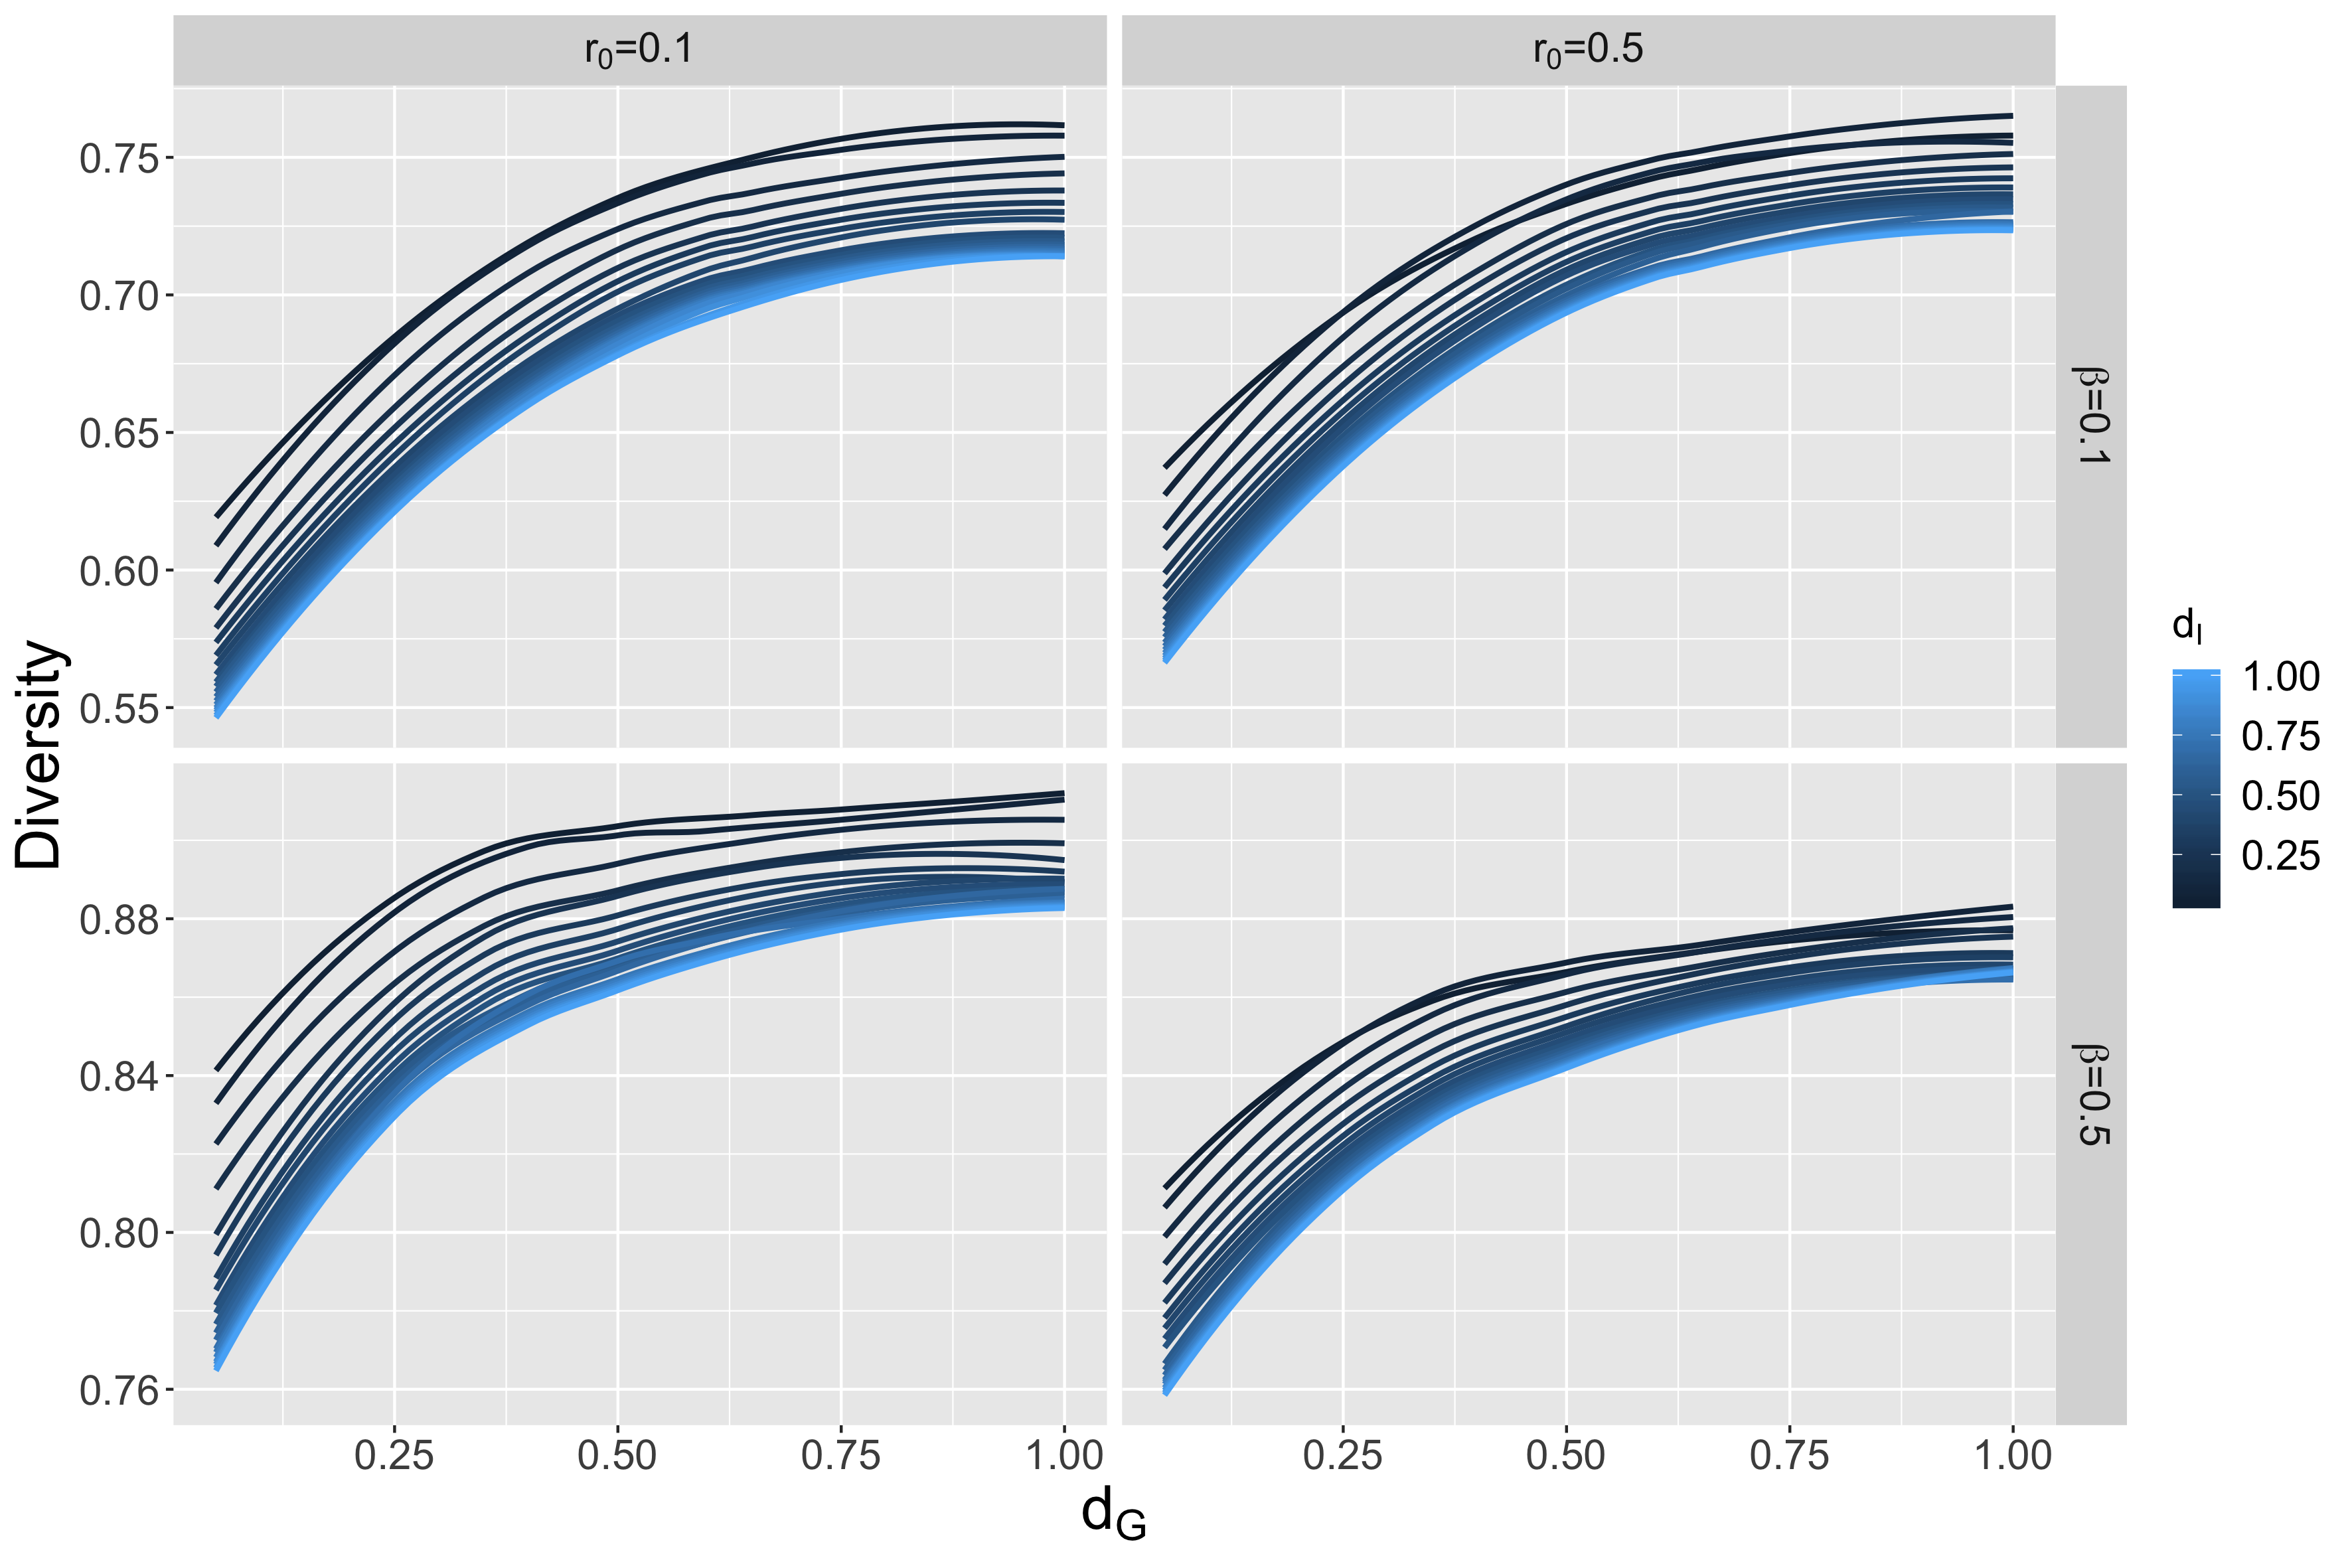
\includegraphics[width=0.7\linewidth]{figures/averageDiversity-gravityDecay_color-innovationDecay_facet-mutationRate-earlyAdoptersRate_newInnovationHierarchy1_utilityStd1_distriblog-normal}
\end{center}

\smallskip

\footnotesize
\textit{Diversity increases with interaction span with a plateau behavior, decreases with innovation diffusion span}

}


\sframe{Model exploration: innovation and hierarchy}{

% Two indicators which behavior is less rich are innovation and population hierarchy (top right and bottom right panels of Fig.~\ref{fig:exploration}), which could be expected as population dynamics are deterministic and strongly related to space, while innovation is directly related to population. We find that these increase both with $d_G$ and $d_I$, meaning that more interactions and more diffusion will foster local innovation. Regarding the final distribution of populations, this implies that systems where interactions are more global will be less unequal. This is however not always the case in such urban dynamics model as explored by \cite{raimbault2020hierarchy}. The mutation rate $\beta$ here only fosters the role of small $d_I$, yielding higher hierarchies and less innovations for these. The effect of initial adoption rate is small for these indicators. Note that although they appear highly correlated in this region of the parameter space, they are not the indicators with the highest correlation as shown further (see Fig.~\ref{fig:cormat} for a correlation matrix between indicators).

\begin{center}
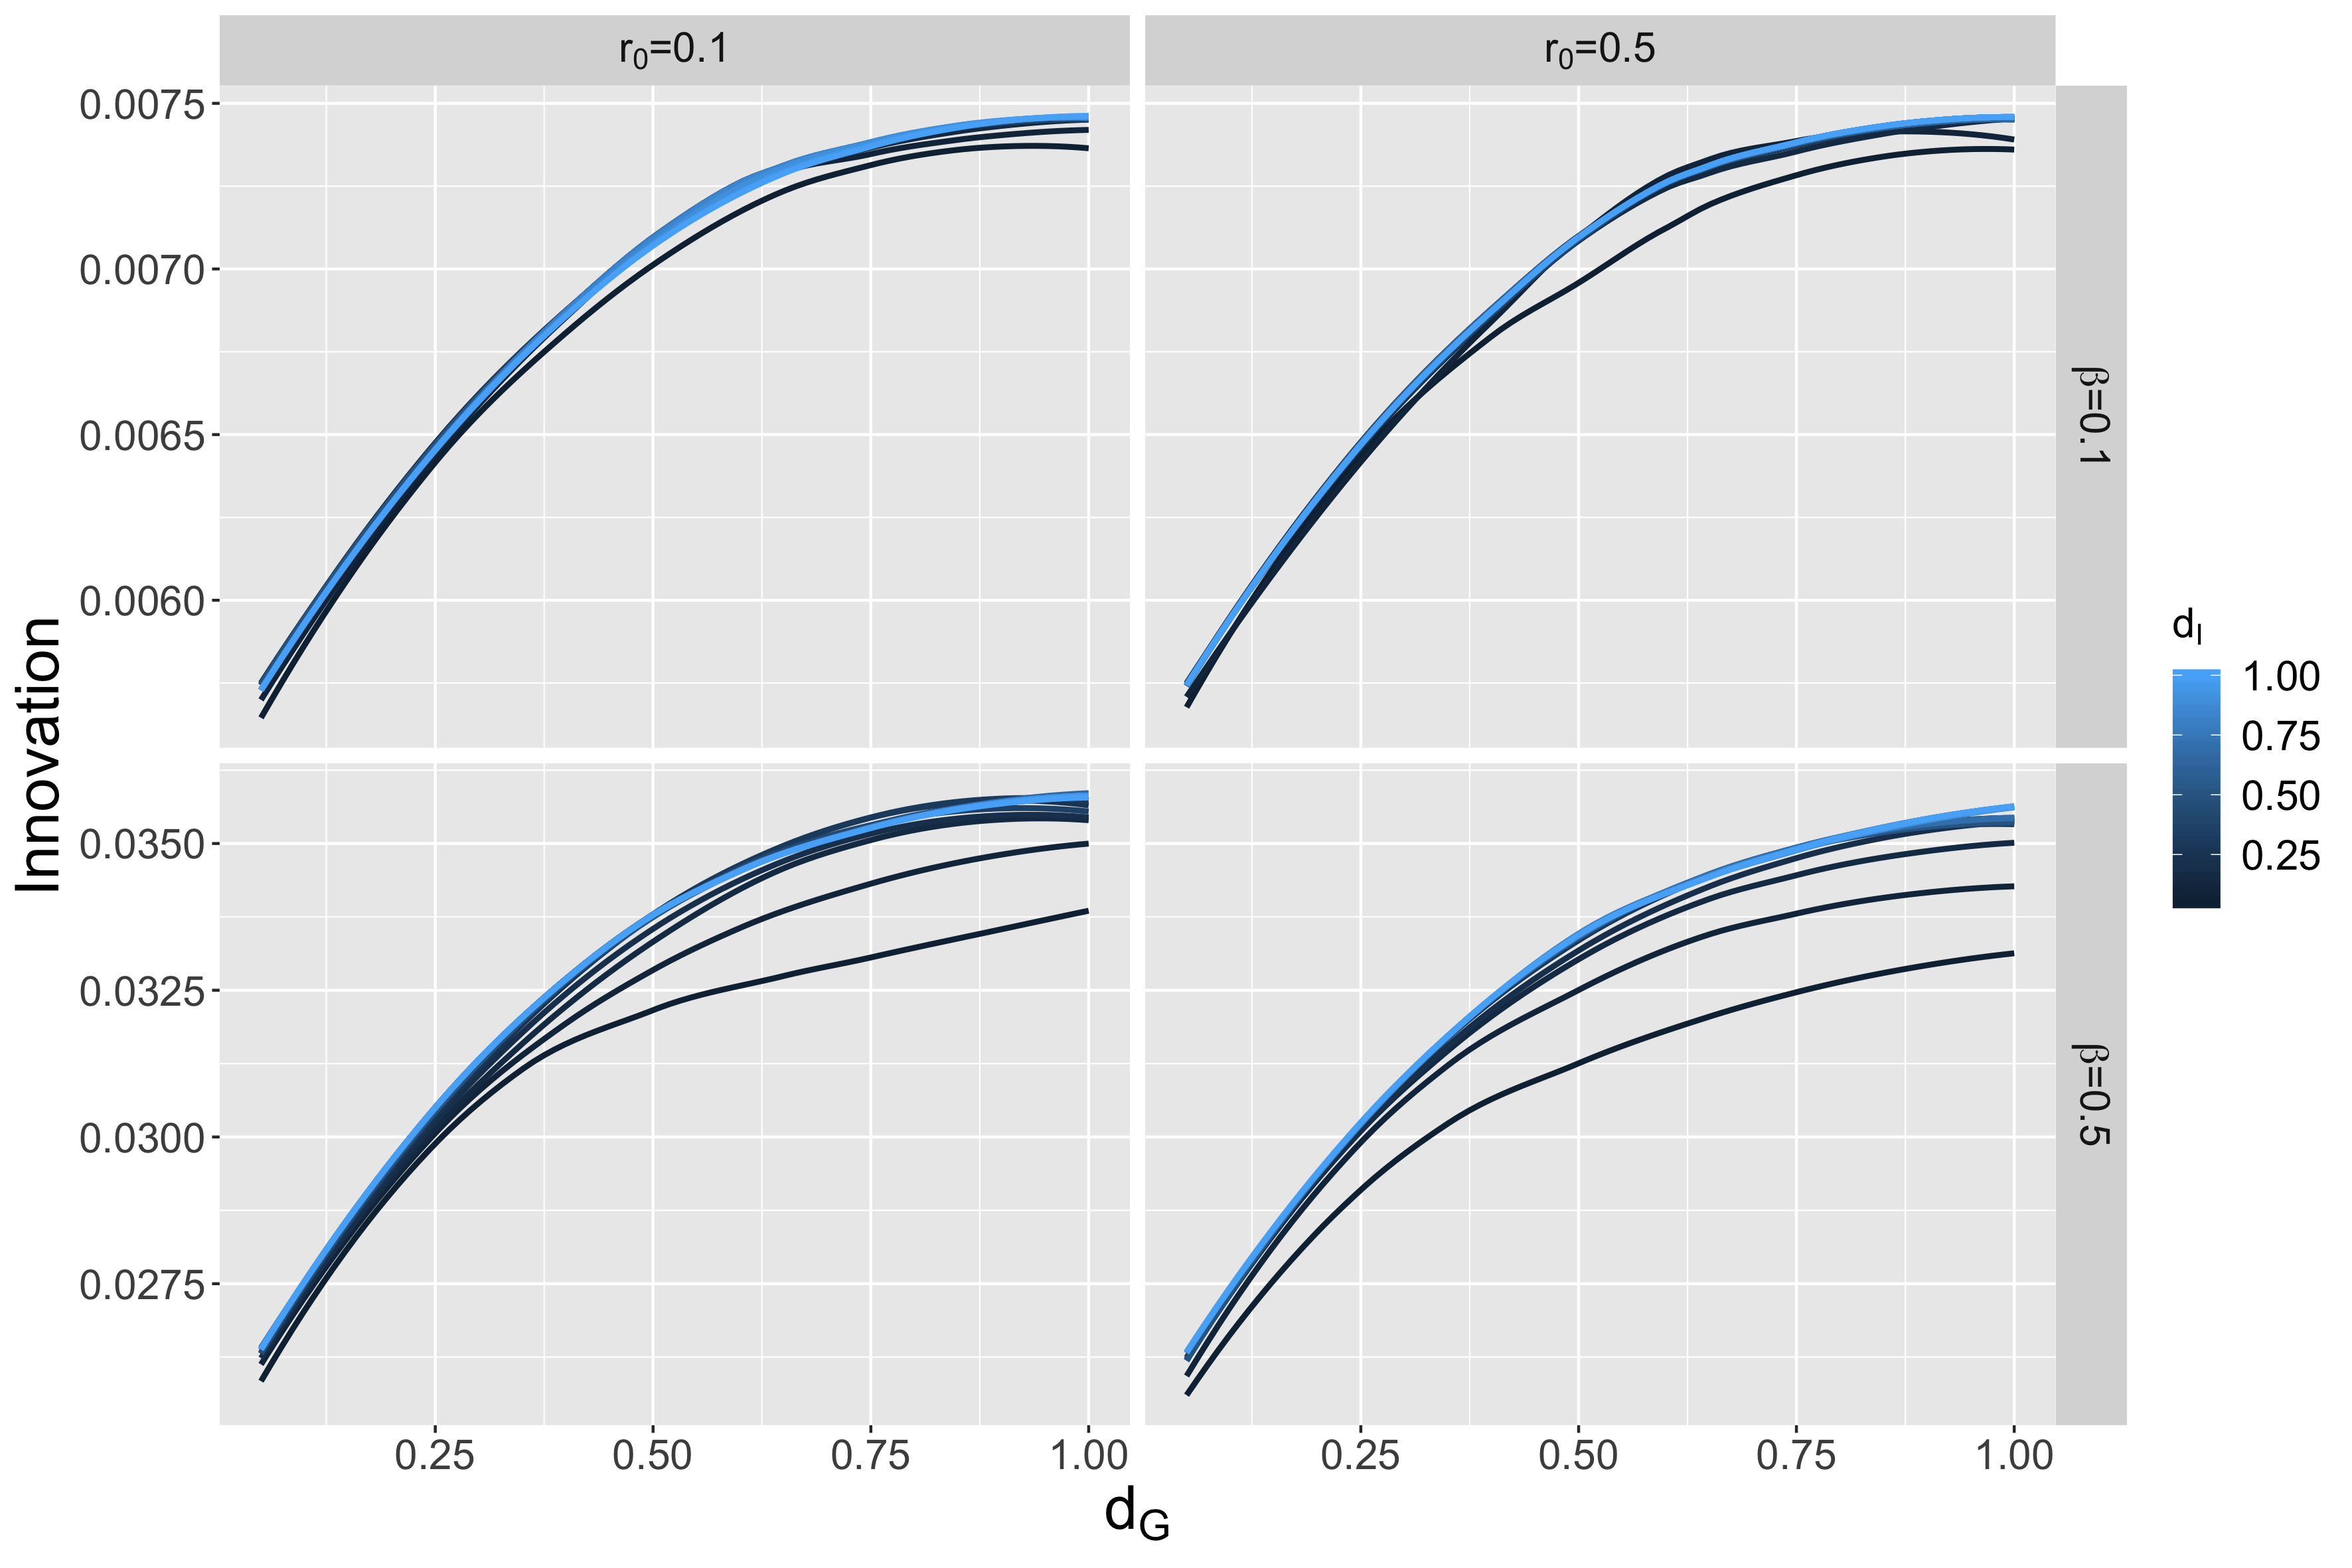
\includegraphics[width=0.47\linewidth]{figures/averageInnovation-gravityDecay_color-innovationDecay_facet-mutationRate-earlyAdoptersRate_newInnovationHierarchy1_utilityStd1_distriblog-normal.png}
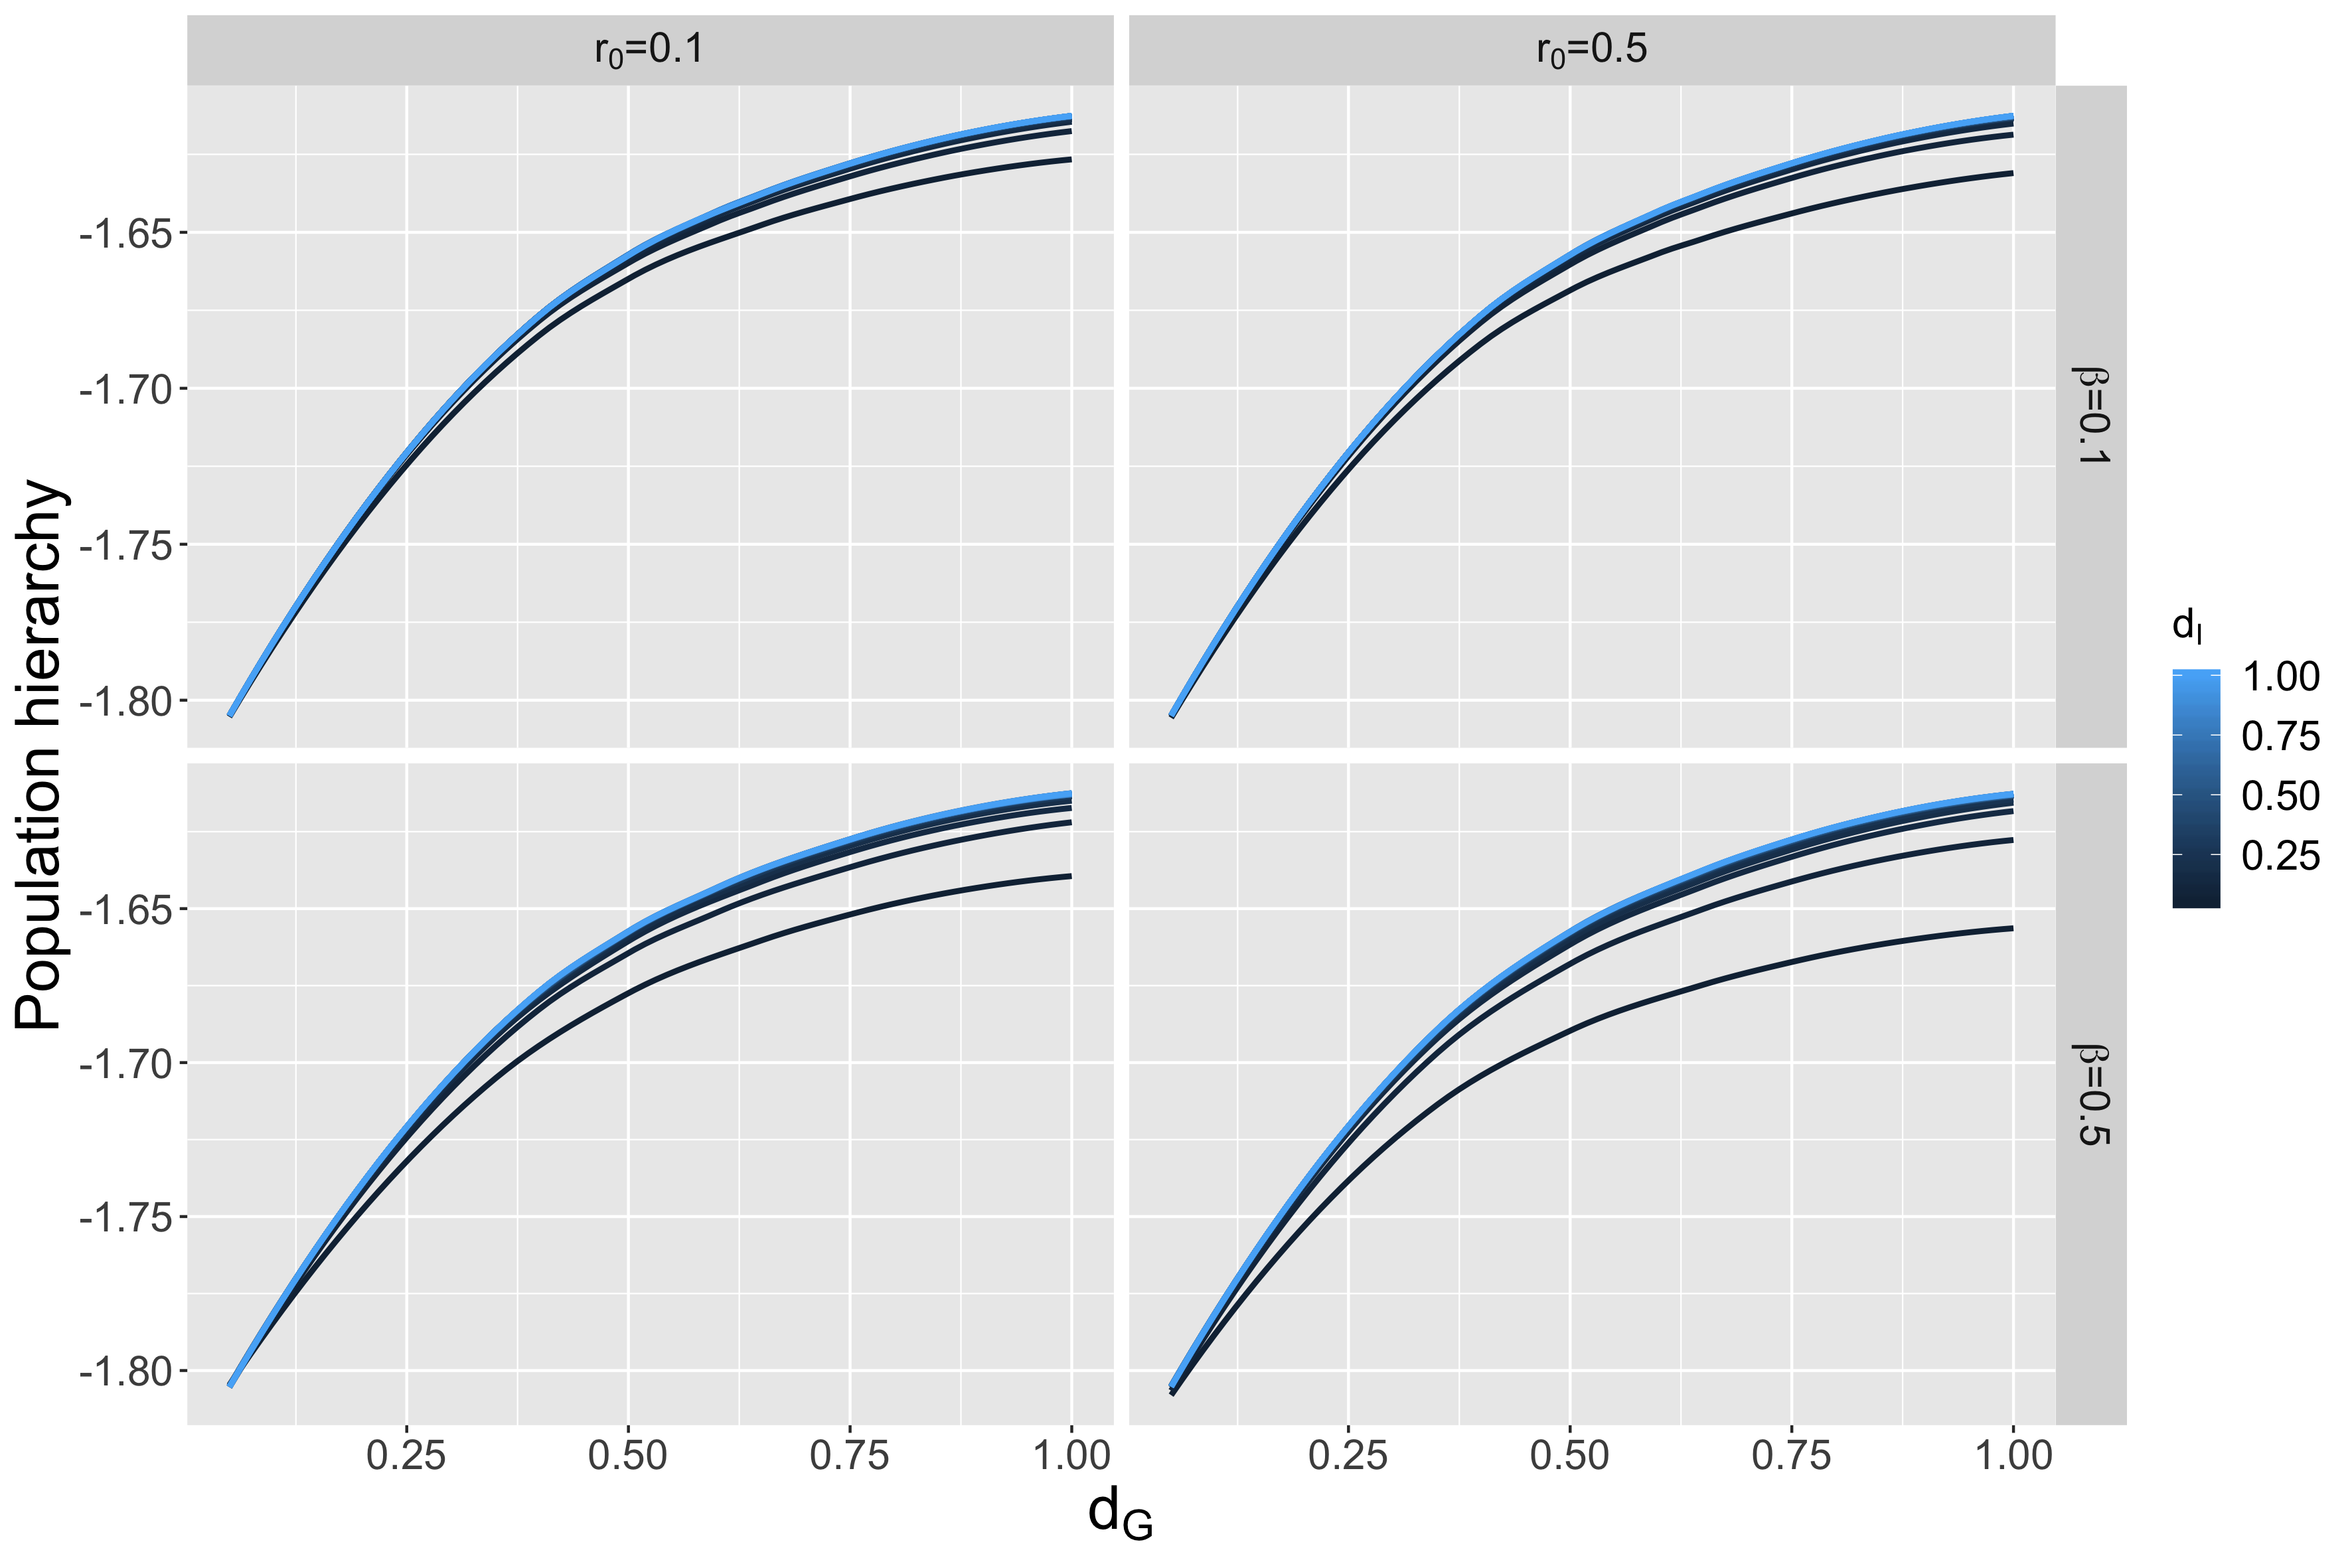
\includegraphics[width=0.47\linewidth]{figures/finalHierarchy-gravityDecay_color-innovationDecay_facet-mutationRate-earlyAdoptersRate_newInnovationHierarchy1_utilityStd1_distriblog-normal.png}
\end{center}

\smallskip

\footnotesize

\textit{Systems with more interactions and diffusion are less unequal and innovate more}

}

\sframe{Model exploration: utility}{

% Finally, the indicator with a more interesting behavior is the utility (bottom left panel of Fig.~\ref{fig:exploration}). For low values of mutation rates, we find a piecewise linear behavior as a function of $d_G$ and small effects of $d_I$, meaning that low innovation settings yield regimes where broader interactions are systematically desirable for the all system. However, when $\beta$ is higher, we witness a maximum of utility as a function of $d_G$, consistent across different values of $d_I$ and of $r_0$. This corresponds to an intermediate regional regime where local innovation regimes are more beneficial than a global integration. This peak is the strongest when innovations diffuse at a broader range, which could be consistent with this regime being due to the emergence of regional ensembles of comparable competitivity. Such a setting would yield a higher chance of introducing innovations with a high utility, while a globalized system would concentrate on a single dominating city and be overall less performant.

\begin{center}
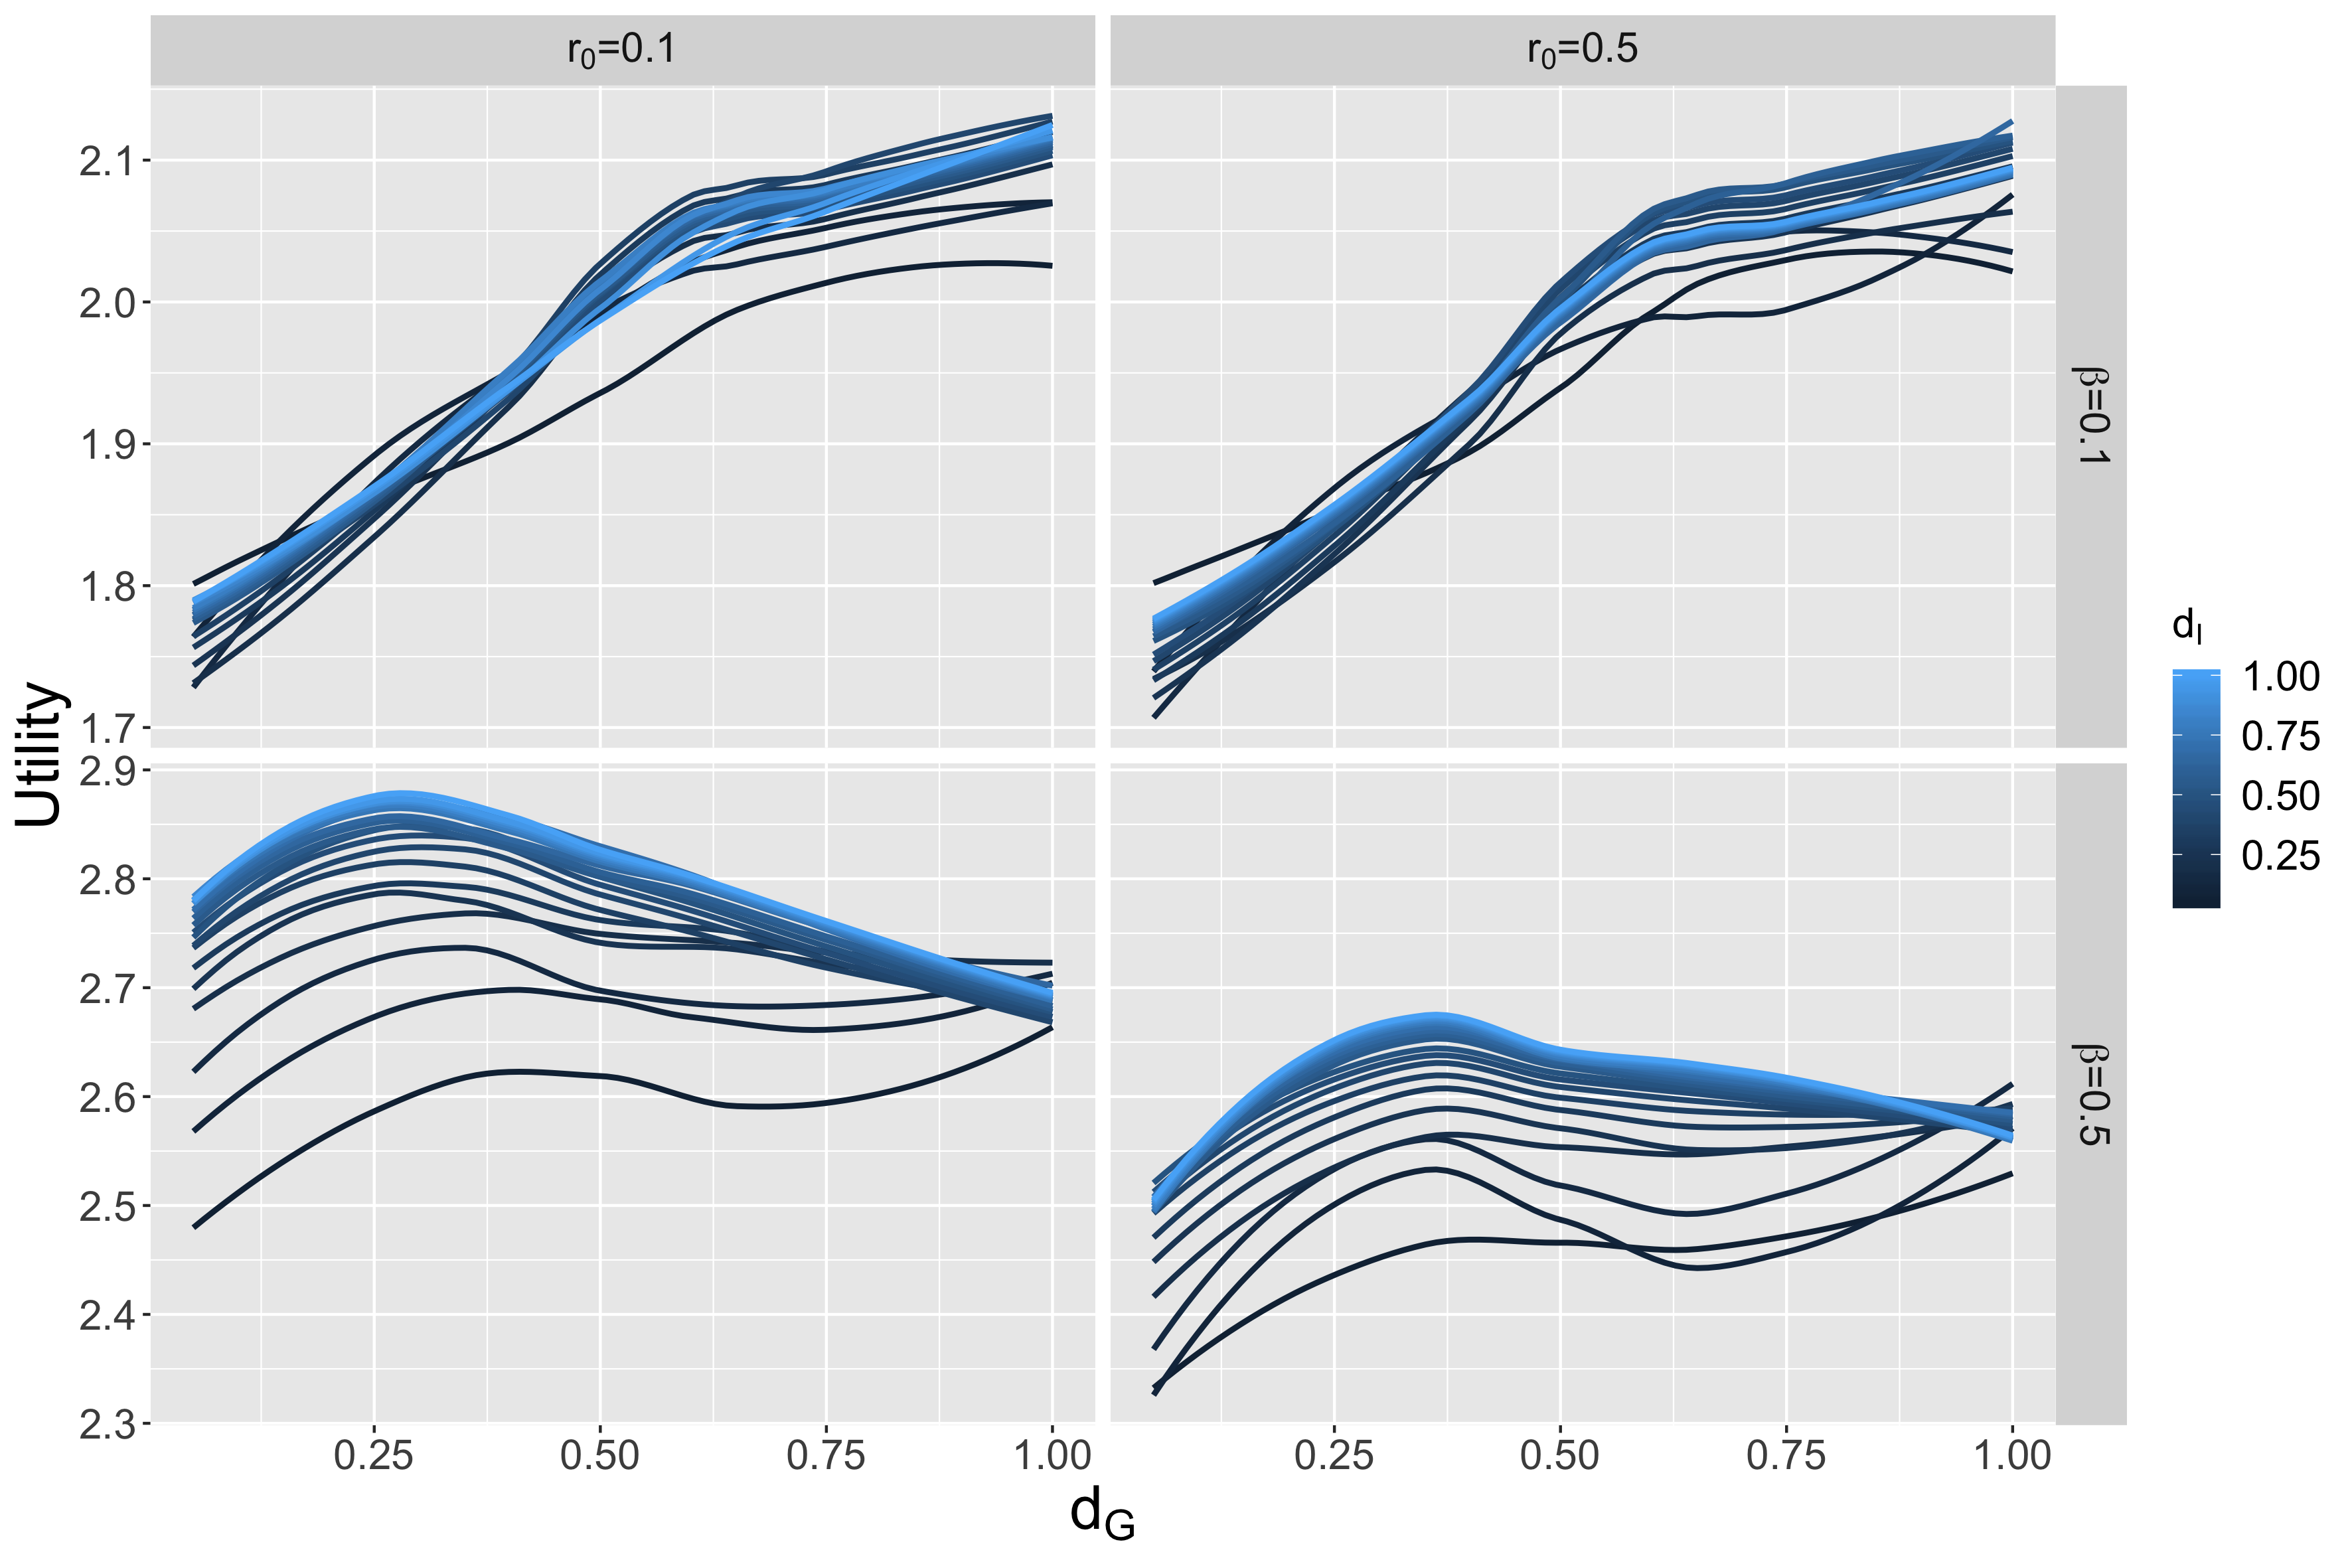
\includegraphics[width=0.8\linewidth]{figures/averageUtility-gravityDecay_color-innovationDecay_facet-mutationRate-earlyAdoptersRate_newInnovationHierarchy1_utilityStd1_distriblog-normal.png}
\end{center}

\footnotesize

\textit{Piecewise behavior for low innovation rates; maximum as a function of $d_G$ for high innovation: emergence of regional innovation clusters?}

}




\sframe{Correlations}{

%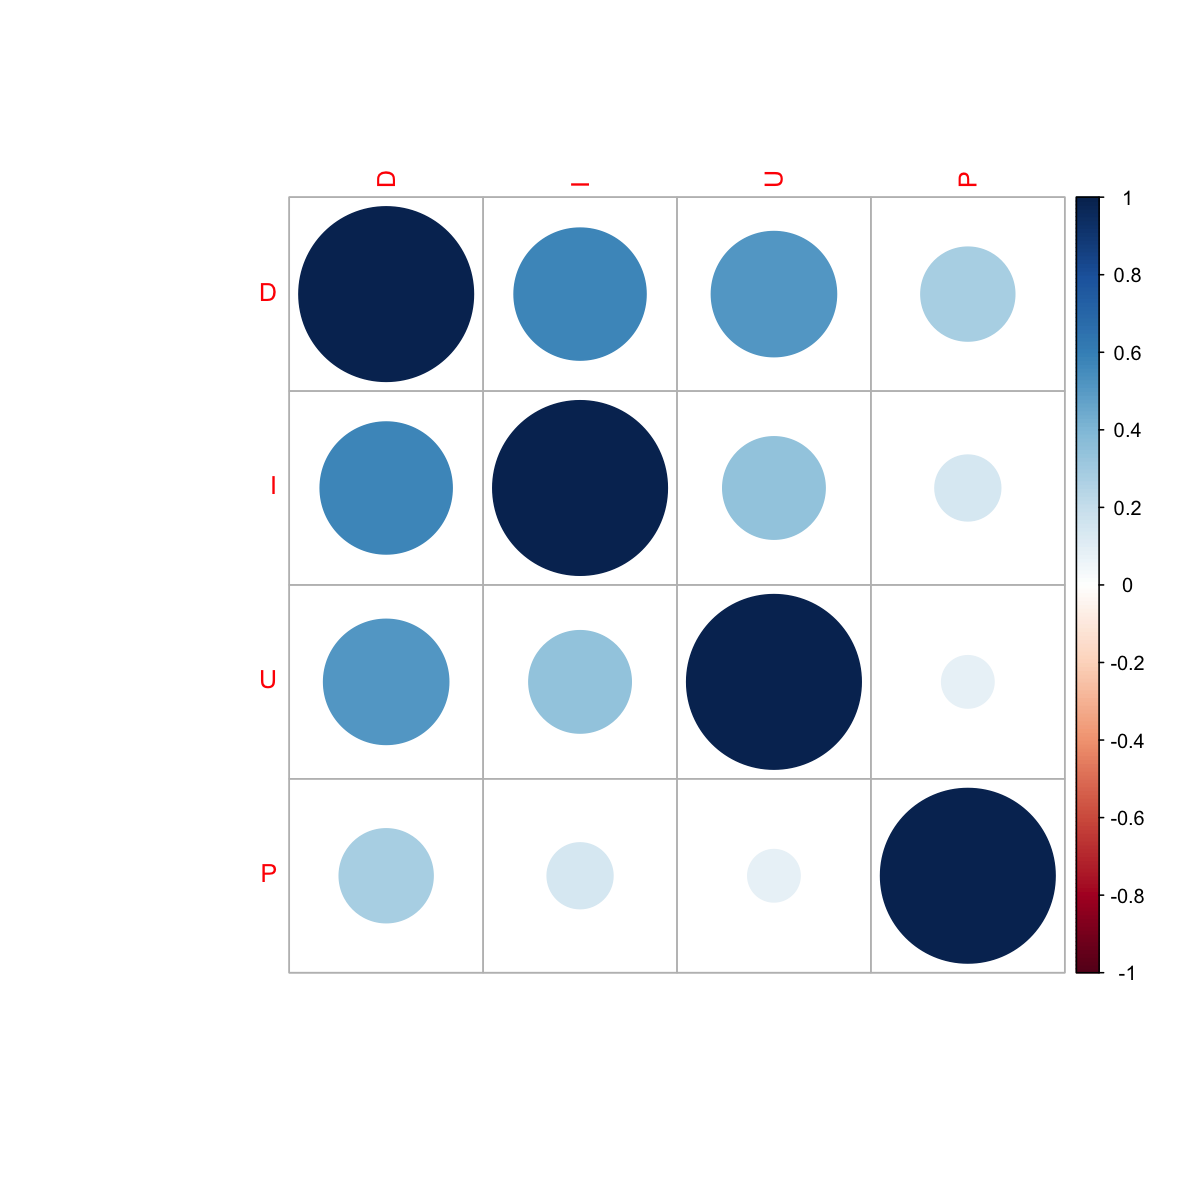
\includegraphics[width=\linewidth,trim={6cm 6cm 0 6cm}]{figures/corrmat_indics.png}
%	\caption{Correlation matrix between indicators, estimated on the full grid experiment. Confidence intervals for correlations estimated with the Fisher method are tiny and not distinguishable in the plot.\label{fig:cormat}}

% We also compute the correlation matrix between indicators across the full grid experiment. This shows that correlations that one could visually extrapolate from studying a part of the parameter space as commented in Fig.~\ref{fig:exploration} do not correspond to the actual correlations on the broader parameter space. Note that local correlation matrices could be estimated for a more thorough discussion. We show the correlation matrix in Fig.~\ref{fig:cormat}. Confidence intervals estimated with the Fisher method are of negligible width compared to correlation values. We find that diversity is finally the indicator with highest correlations. The correlation between innovation and population is low, meaning that the similar curves observed before are a particular case. Innovation and utility have a correlation lower than 0.5, and are thus rather independent. Regarding the effective dimension of the indicator space, a principal component analysis on normalized indicators gives 48\% of variance on the first component, 77\% of cumulated variance on the second and 91\% on the third. This confirms that even if correlations exist, the behavior of indicators are rather independent.

\begin{center}
	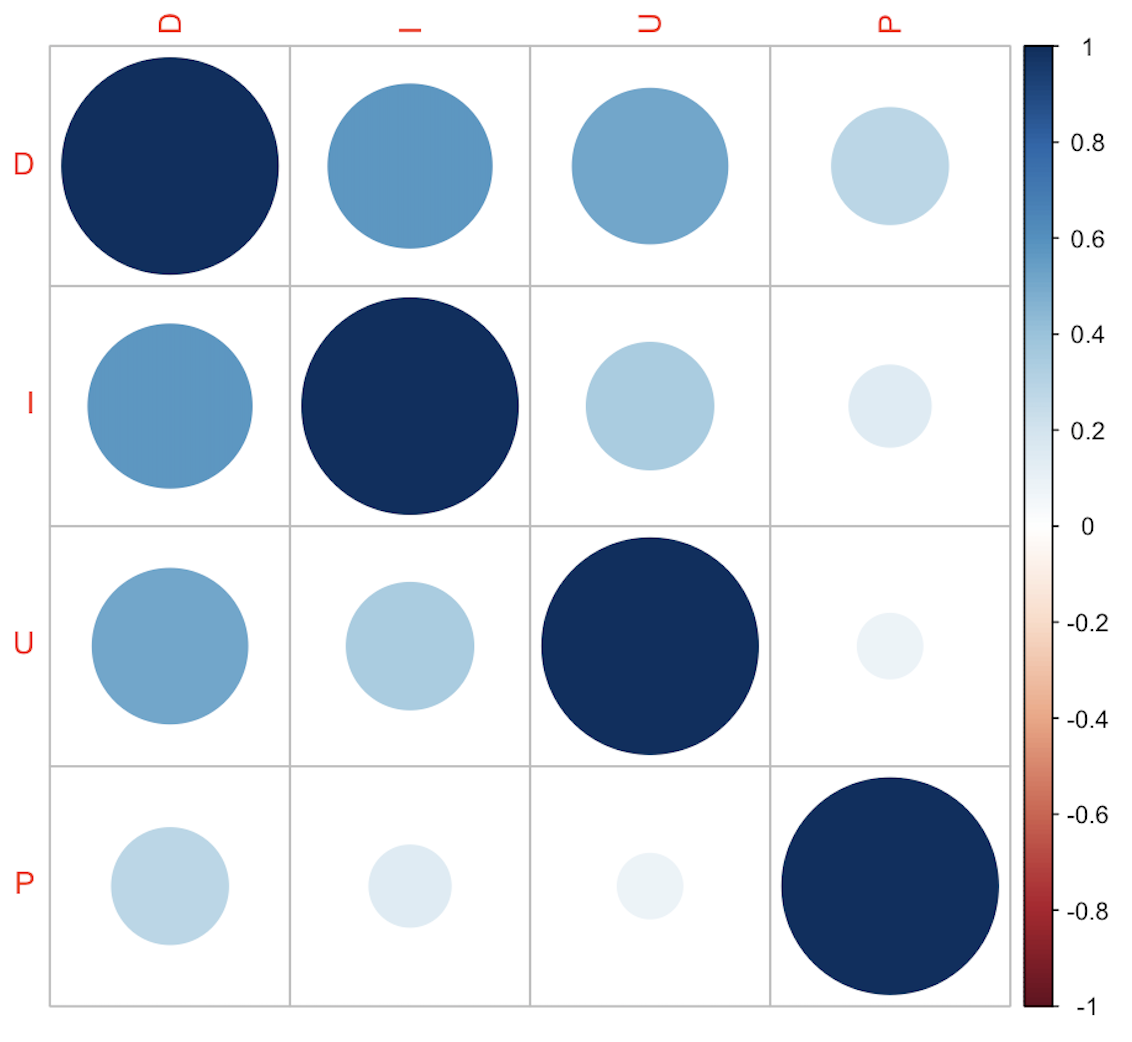
\includegraphics[width=0.6\linewidth]{figures/corrmat_cropped.png}	
\end{center}

\footnotesize

\textit{Correlation matrix estimated over the whole exploration: innovation and population are not strongly correlated; 91\% of variance on first two components}

}


\sframe{Model optimization}{


% 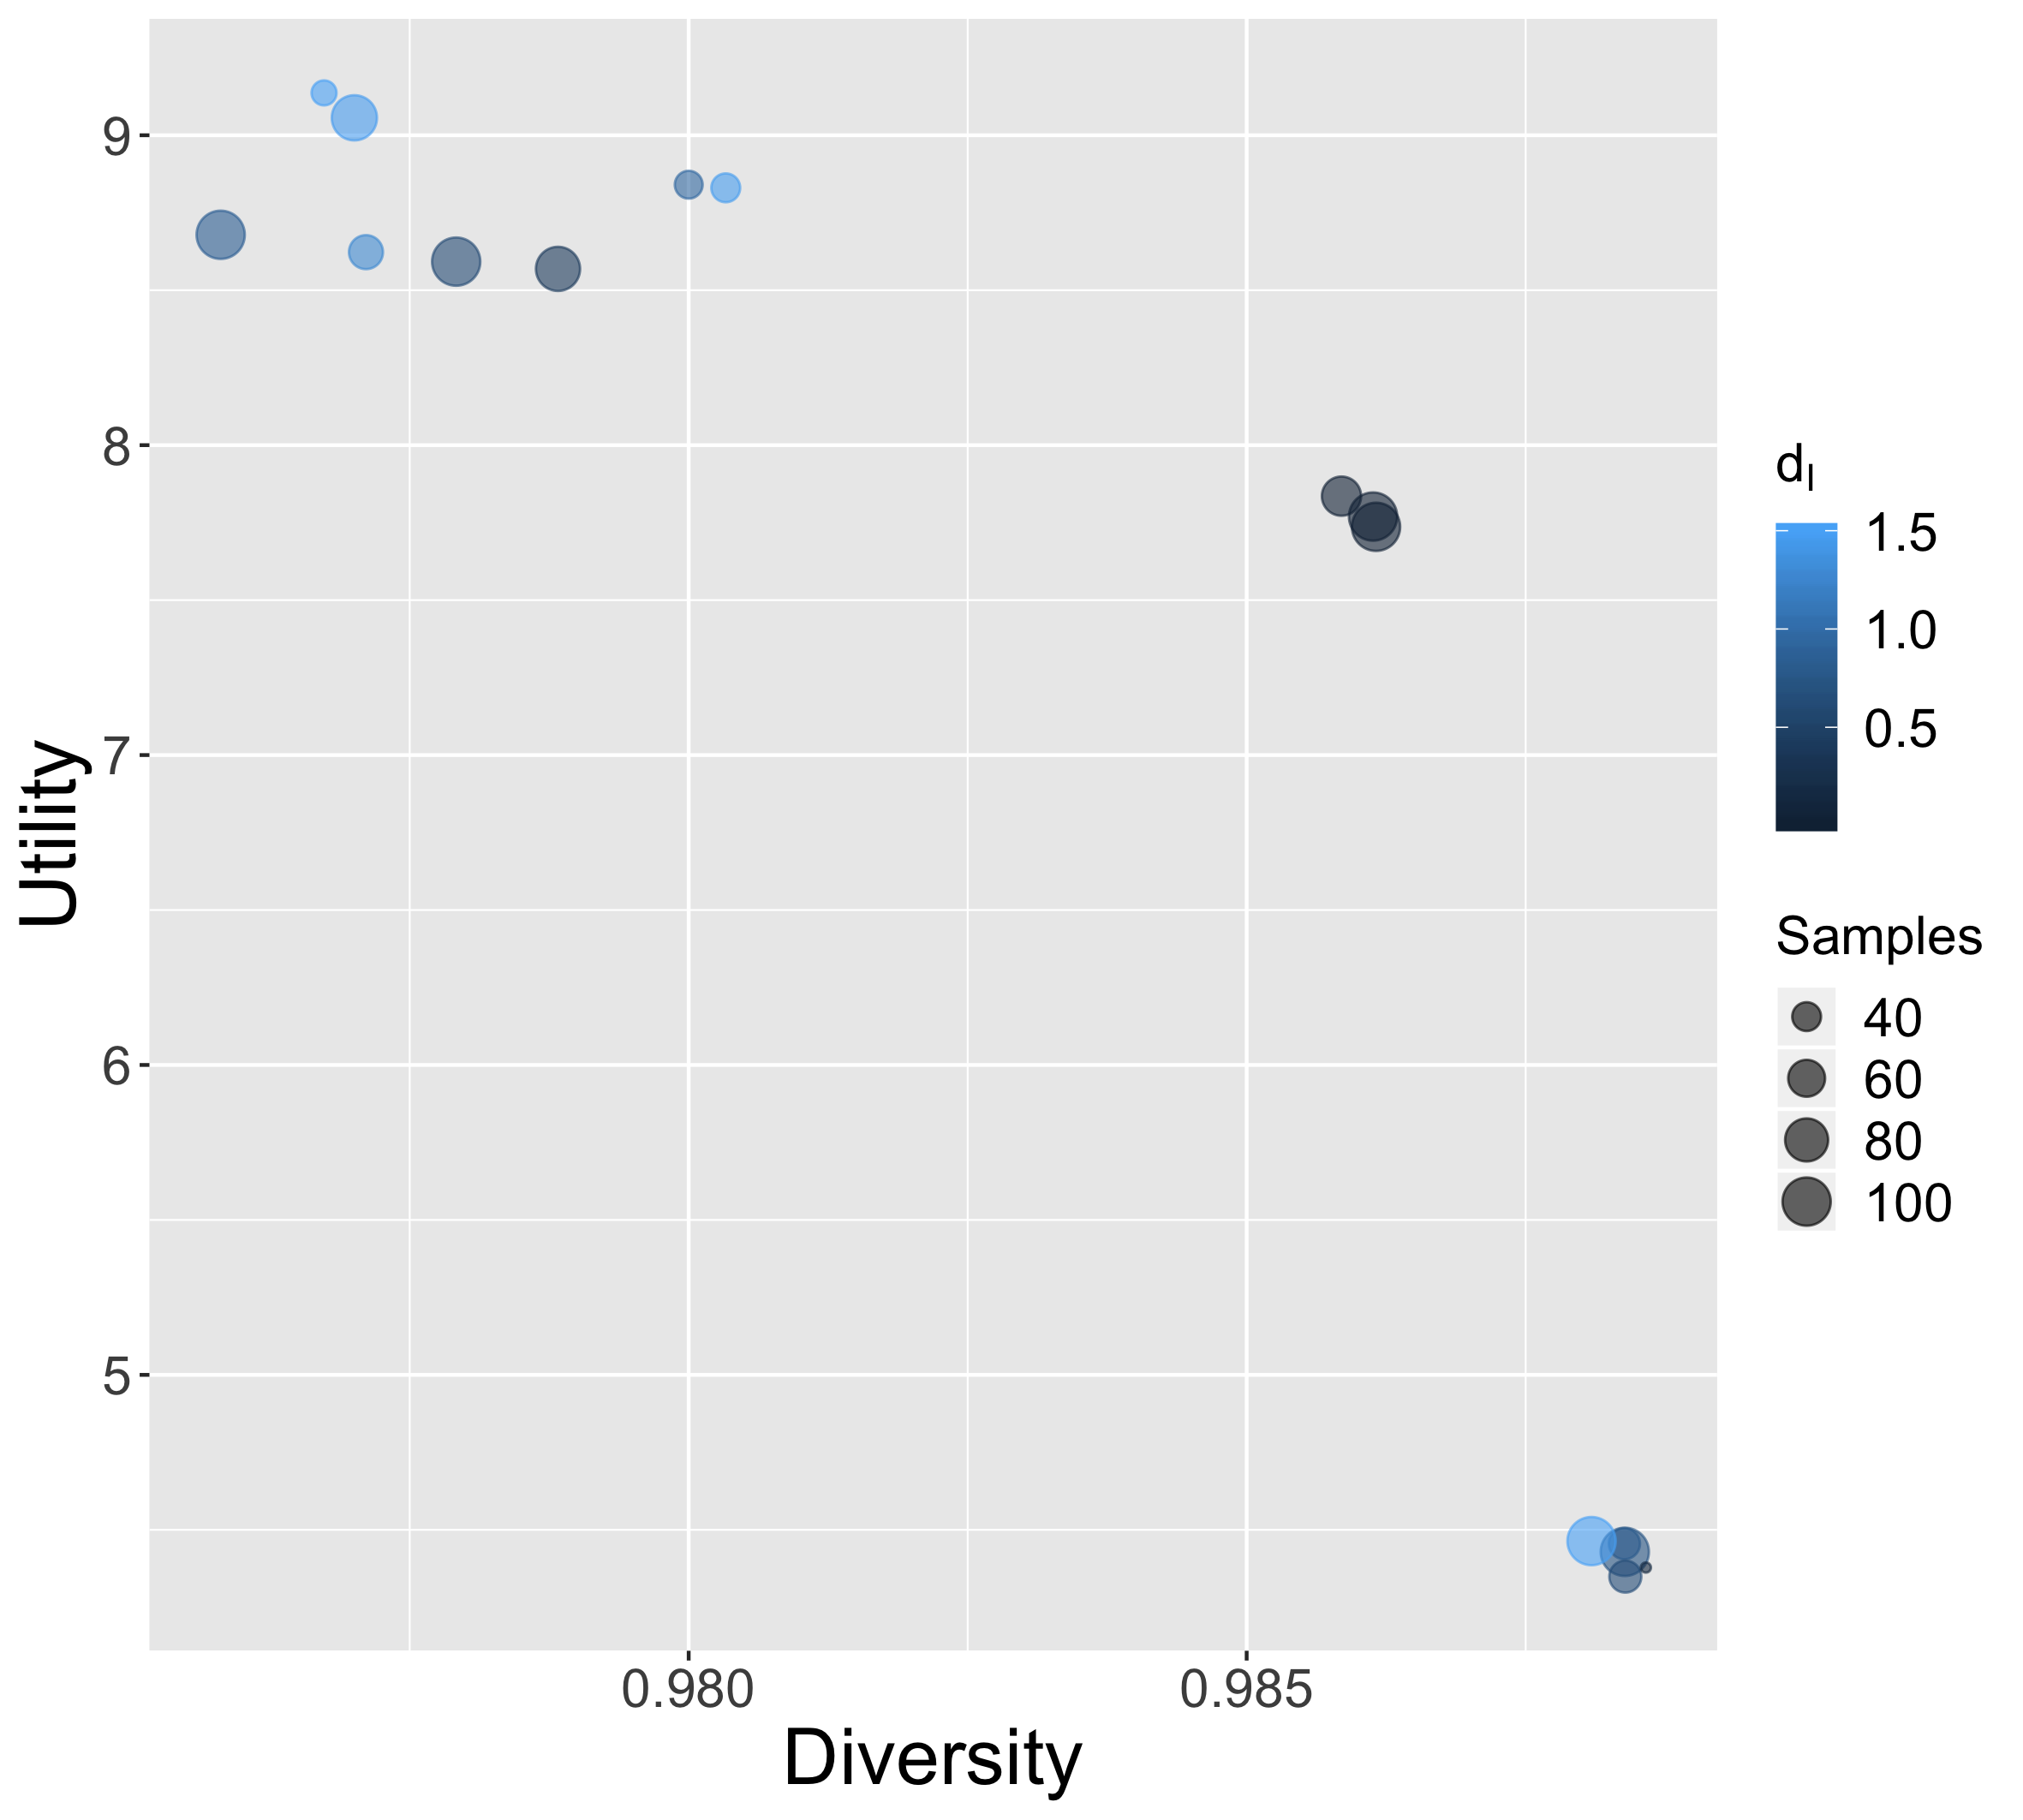
\includegraphics[width=\linewidth]{figures/paretoDiversity-Utility_colorinnovationDecay.png}
%	\caption{Pareto front for the contradictory indicator of utility and diversity obtained with the NSGA2 algorithm. Point color gives innovation interaction range $d_I$ while point size gives the number of stochastic samples.\label{fig:pareto}}

% The last experiment we perform is the application of a multi-objective optimization procedure to the model. More particularly, one could want to optimize simultaneously the global utility but also the diversity to ensure a certain resilience in the urban system. We apply thus a bi-objective genetic algorithm on the model, trying to maximize simultaneously utility and diversity. The algorithm is the NSGA2 algorithm \citep{deb2002fast}, which we run for 50,000 generations with a population of 200 individuals and an Island distribution scheme. The algorithm is integrated into the OpenMOLE software, and the stochastic aspect is internally tackled by using an embedding strategy, i.e. by adding the number of repetitions as an additional objective to find compromize points between the number of run needed and their statistical accuracy.
%We show in Fig.~\ref{fig:pareto} the obtained points, which are close to a Pareto front. We include the points with at least 20 stochastic samples. We find three regimes, the first corresponding to the upper points in the plot for higher utilities but lower diversities, which should correspond to the intermediate optimal regimes identified before, and in which some kind of linear compromize between utility and diversity exists (but with a very flat slope for utility): increasing global utility is done at the cost of reducing diversity. Within this first regime, two very different parameter setting coexist, one with high innovation diffusion (light blue, points with higher utility), the other in dark blue with a more local innovation diffusion. This means that reducing the span of innovation diffusion will increase diversity as one could expect. A second part of the Pareto front corresponds to intermediate points with lower utility but higher diversity, and is exclusively composed of local innovation parameters. The third part of the Pareto front, obtained after a sharp transition, allows increasing significantly the diversity compared to the first part, but at the price of a much lower utility (points on the bottom right). These points are all close to equivalent, and one may prefer to consider as a compromize the extreme points which correspond to a broad diffusion setting, but this last regime is also mixed with local innovation. Thus, local diffusion correspond to intermediate compromizes, while broad diffusion corresponds to extremes in the Pareto front (first and third regimes). In a nutshell, this optimization exercise is interesting both to show how the model produces compromizes, but also how it could be used in practice for innovation policies applied to systems of cities.

\begin{center}
	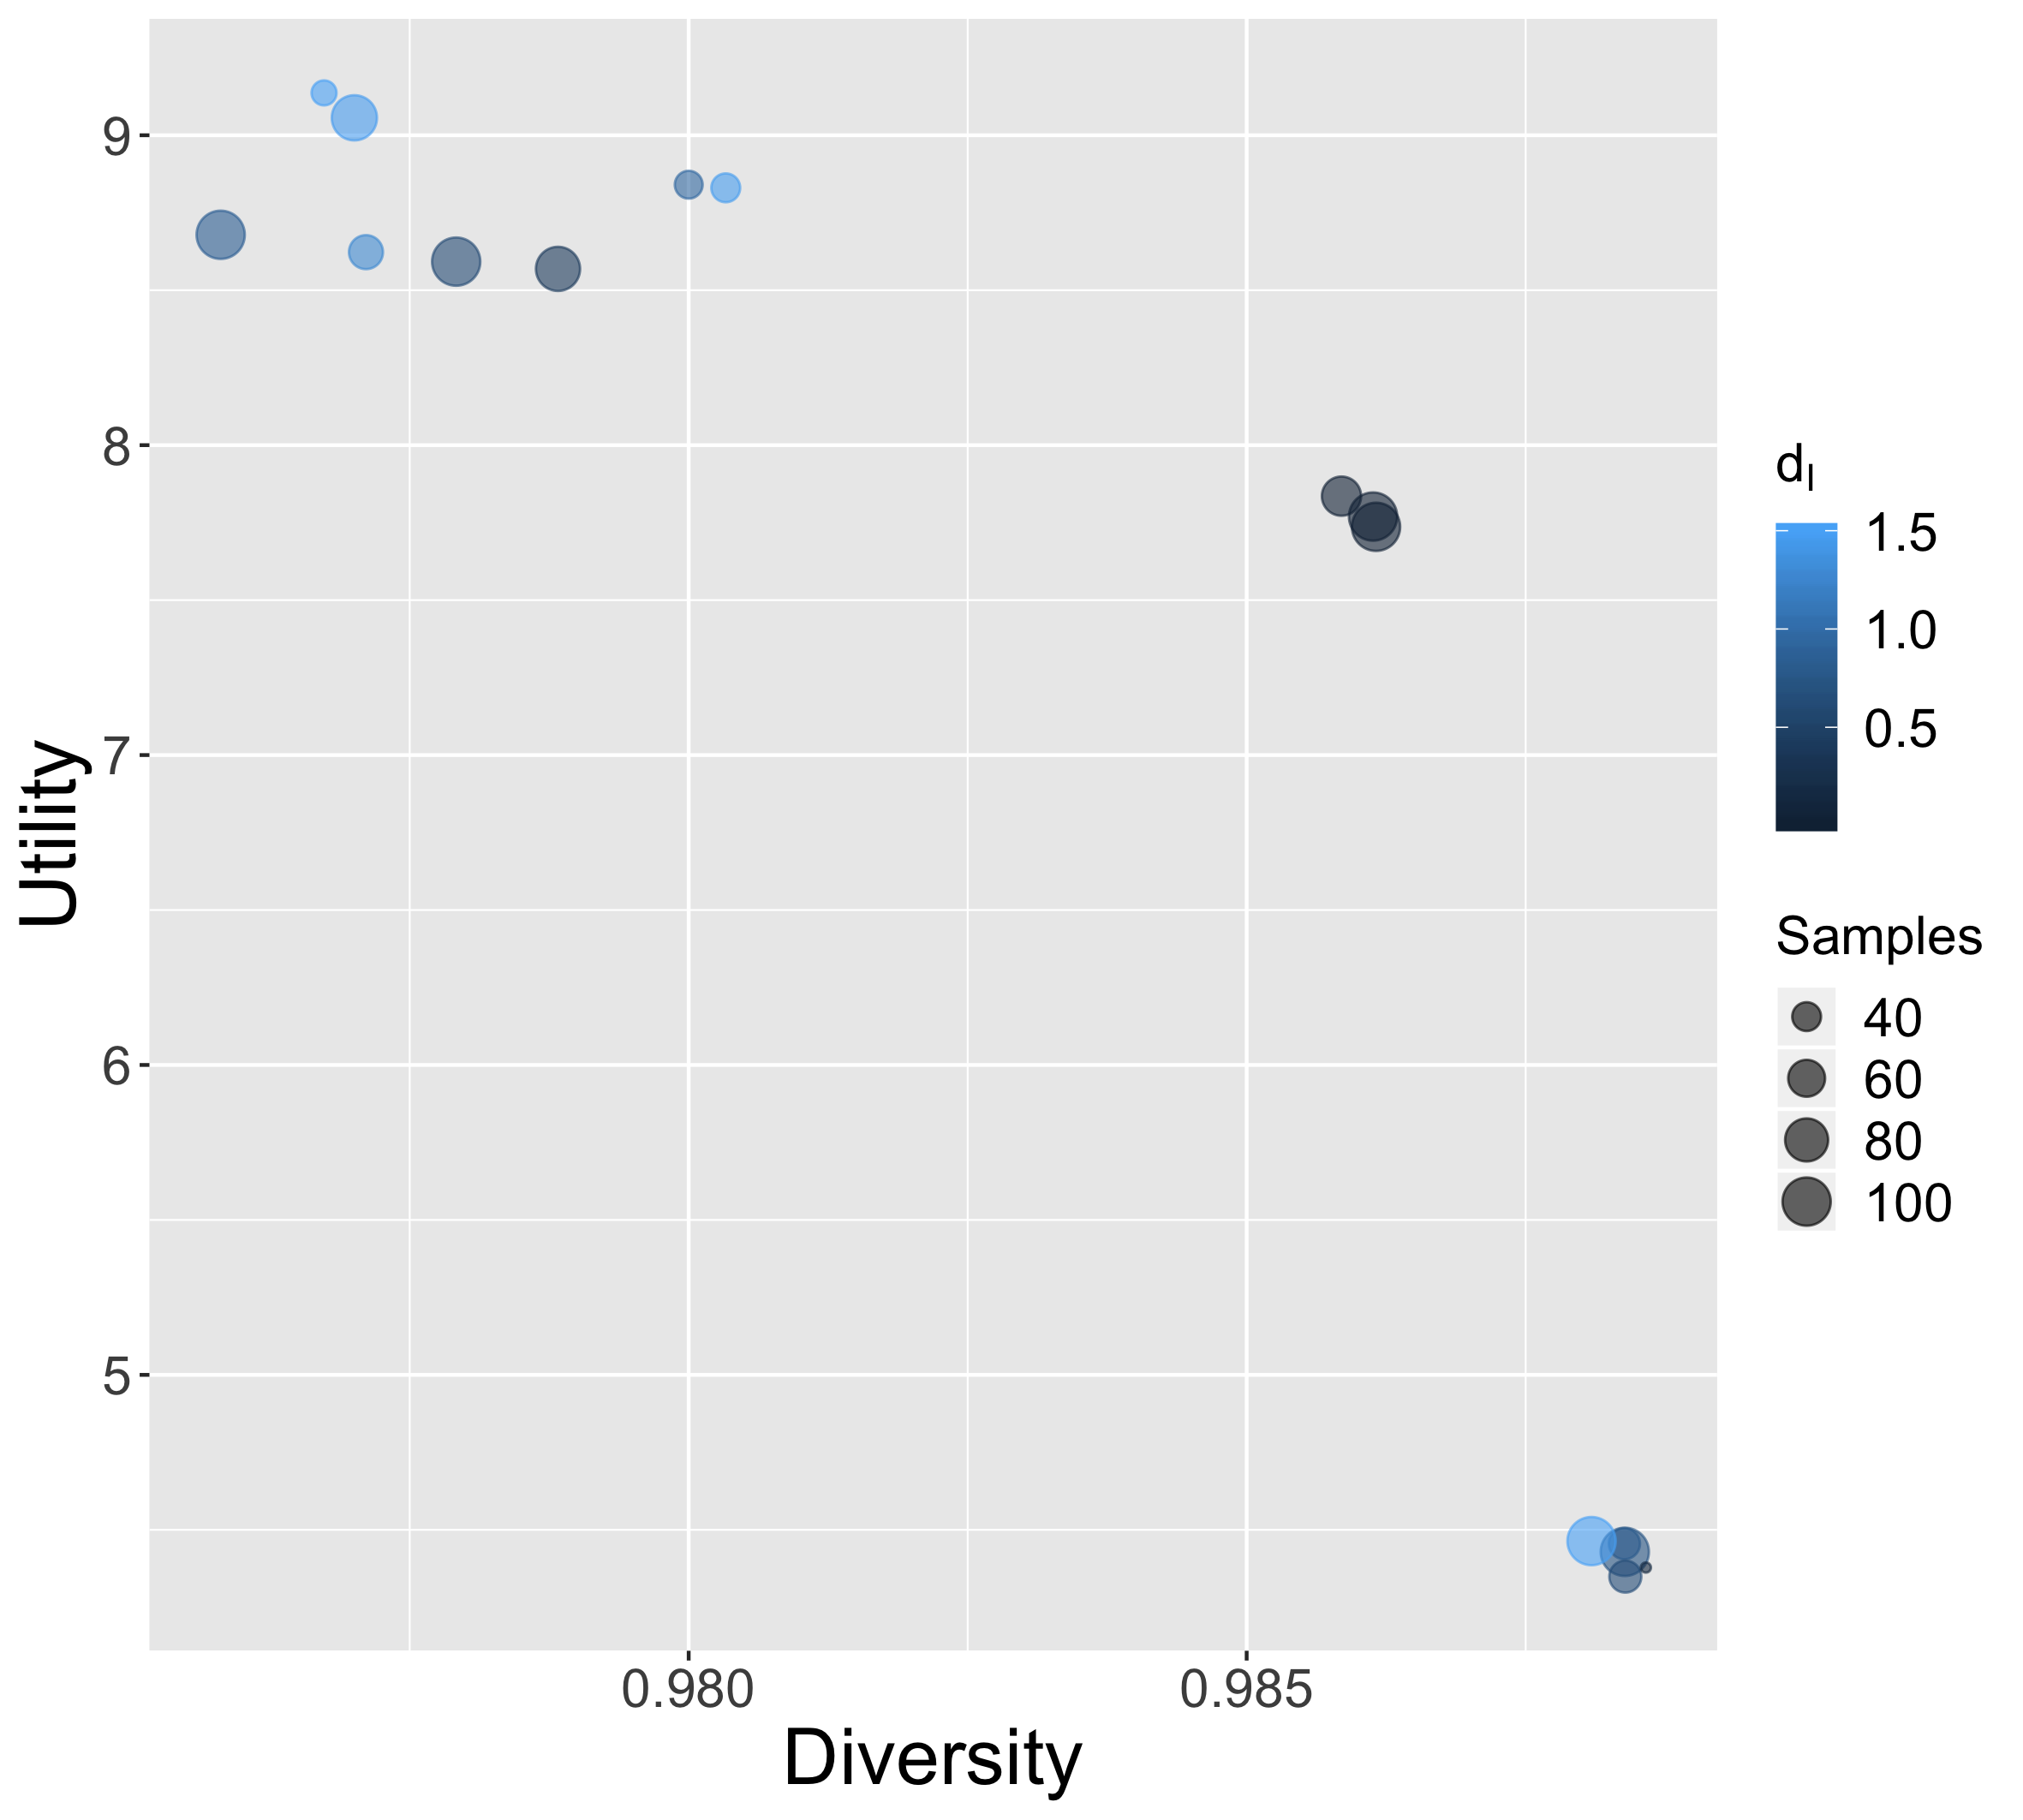
\includegraphics[width=0.6\linewidth]{figures/paretoDiversity-Utility_colorinnovationDecay.png}
\end{center}

\footnotesize

\textit{NSGA2 algorithm to simultaneously optimize utility and diversity: emergence of three compromize regimes; intermediate regime with low level of innovation diffusion}




}




\section{Discussion}



\sframe{Discussion}{

% Our simple formulation of an urban genome and associated evolutionary processes, implemented by the diffusion of innovation, already capture complex urban dynamics, as shown for example by the emergence of an intermediate optimal regime corresponding to local innovation niches which diffuse far. Although much more empirical work would be needed to compare these stylized facts to real world settings, our model suggests in this particular setting that too much integration is not always optimal, what corresponds to the theoretical fact that complex systems are generally modular at different scales \citep{ethiraj2004modularity}. More generally, regarding the implications of our results for possible formalizations and theories of urban evolution which would closely build on biological and cultural evolution by extending them, we have demonstrated how a particular instance of an urban genome can be used to simulate urban dynamics, including fundamental processes needed to effectively have evolution. To what extent this approach relates to existing approaches of urban evolution which use other definitions remains to be investigated.

%Several extensions and applications would be possible to this first model exploration. First, the innovation space in our model remained unidimensional. \citep{hidalgo2007product} show in terms of industrial production by countries that these industrial spaces are highly dimensional in terms of product produced and interdependencies between countries and types of production, increasing the path-dependency in economic trajectories. The investigation of patent data from a semantic viewpoint also shows the highly dimensional nature of technological innovation \citep{raimbault2016investigating,bergeaud2017classifying}. A direct extension of our model would consist in having a matrix genome instead of a vector one. Innovations would occur across several dimensions which can correspond to industrial or technological domains, but also social and cultural innovation and innovations in terms of infrastructures which condition the way systems of cities evolve \citep{raimbault2018caracterisation}. Each dimension should have particular innovation rules depending on its nature, and dependencies across dimensions could be introduced, implementing the possible emergence of technological co-evolution niches beside the spatial co-evolution niches.

%Second, applying the model to real systems of cities, both in terms of initial parametrization and of empirical laws for innovation processes, would allow bringing this approach closer to possible policy applications. \cite{raimbault:halshs-01880492} and later \cite{2020arXiv200510007R} benchmarked several models of urban growth based on interactions between cities, and integrated the model of \cite{favaro2011gibrat} on which this work was based. It however only included accurate initial populations and distance matrix, but no empirical data on innovation waves which were also synthetically constructed. One important aspect of this application to real systems of cities is thus a test of the performance of this model in predicting possible population trajectories for systems of cities. Several obstacles however remain for a more complete application of the innovation diffusion urban evolution model. Harmonized datasets with consistent definition of urban entities, in particular which can be compared between different urban systems and long time scales, are crucial to study the dynamics of urban systems as done for example by \cite{pumain2015multilevel}. Innovation measures are not included in such datasets, and existing innovation proxys are limited in time and space, as for example the US Patent Office database for which inventors have been localized \citep{morrison2017disambiguation}. Then, how to link innovation proxy measures with model processes, in other words how to parametrize or calibrate the model on real data, remains an open question. Finally, how various urban systems with very different histories and at different stages of development would fit model assumptions, in particular the fact that innovation waves partly drive growth rates of cities, remains to be empirically investigated \citep{pumain2009innovation}.

%Finally, our approach was rather restricted in the sense that even a broad geographical range is taken into account, a single ontological scale is included in the model, i.e. the macroscopic scale since cities are the basic agents. One can expect processes of innovation diffusion to behave differently at the microscopic scale or at intermediate scales of companies or innovation clusters \cite{audretsch2004knowledge}. Other types of agents and processes may be more significant than spatial interaction at this finer scales, for example with a diffusion through social networks \citep{zhang2019empirically}. Similarly, a single temporal scale was included, although two dynamics of spatial interaction and innovation diffusion are effectively combined. A multi-scale approach of urban evolution would be necessary to fully account for the complexity of these systems. \cite{raimbault:halshs-02351722} introduced a multi-scalar model for population growth with upward and downward strong feedbacks between the mesoscopic scale (urban form) and the macroscopic scale (spatial interaction model). Adapting this approach in the case of urban evolution through innovation diffusion would be an interesting potential development.

\textbf{Empirical and theoretical implications}

\smallskip

$\rightarrow$ Global integration of cities is not necessarily optimal in terms of overall utility

\smallskip

$\rightarrow$ Urban evolution simulation model including explicit evolution processes and an urban genome

\medskip

\textbf{Future work and extensions}

\smallskip

$\rightarrow$ Multi-dimensional urban genome to capture multi-dimensionality of urban dynamics \cite{hidalgo2007product}

\smallskip

$\rightarrow$ Application to real systems of cities \cite{2020arXiv200510007R}: patent data as possible proxy for innovation dynamics \cite{bergeaud2017classifying}

\smallskip

$\rightarrow$ Processes at other scales, towards multi-scale models \cite{raimbault:halshs-02351722}


}




\sframe{Conclusion}{

% We have introduced a simple model of urban evolution integrating effectively the evolutionary processes of transmission, transformation and evolving sub-systems, through innovation diffusion and spatial interactions. Model exploration yield complex behavior while multi-objective optimization shows the potentiality for the model to produce compromizes between utility and diversity in the system of cities. This work is thus a first step towards more elaborated models of urban evolution.


$\rightarrow$ A simple model of urban evolution capturing complex dynamics at the macroscopic scale through the diffusion of innovations

\medskip

$\rightarrow$ An ALife approach to the simulation of urban systems: ``Cities as they could be''


\bigskip
\bigskip

\footnotesize

\textbf{Open repositories for}

\begin{itemize}
 \item Model and results: \texttt{https://github.com/JusteRaimbault/UrbanEvolution}
 \item Simulation data: \texttt{https://doi.org/10.7910/DVN/Q5GKZ0}% dataverse
\end{itemize}

\bigskip

\textbf{Acknowledgments}: thanks to the \textit{European Grid Infrastructure} for access to the infrastructure; UKCRIC DAFNI and Urban Dynamics Lab Grant EPSRC EP/M023583/1 for funding


}





%%%%%%%%%%%%%%%%%%%%%
\begin{frame}[allowframebreaks]
\frametitle{References}
\bibliographystyle{apalike}
\bibliography{biblio}
\end{frame}
%%%%%%%%%%%%%%%%%%%%%%%%%%%%










\end{document}

